% ============================================================================
%  TRADUCCIÓN DE TRABAJO AL ESPAÑOL — NO ES EL MANUSCRITO DE RECORD
%
%  Fuente:  docs/paper/nowcast-ems.tex
%  Commit:  eef6202  (sha del .tex: ver la línea \sourcehash de abajo)
%  Fin:     auditoría del contenido en la lengua del autor.
%  Nota 2026-10-07: el inglés tuvo una revisión de ESTILO (registro, oraciones
%  partidas, incisos) sin cambio de contenido ni de cifras; esta traducción
%  refleja el contenido y las cifras de ese commit, no su redacción literal.
%
%  REGLA DE ORO: ante cualquier discrepancia manda el .tex en inglés.
%  Este archivo NO se somete, NO se cita y NO debe editarse para corregir el
%  paper — las correcciones van al inglés y esta traducción se regenera.
%
%  Notación numérica: se preserva EXACTAMENTE la del original (punto decimal,
%  no coma) para que las cifras se puedan comparar máquina contra máquina.
%  Ver scripts/check_translation_numbers.py.
% ============================================================================
\documentclass[authoryear,preprint,review,12pt]{elsarticle}

\usepackage[T1]{fontenc}
\usepackage[utf8]{inputenc}
\usepackage[spanish,es-noshorthands,es-nodecimaldot]{babel}
\usepackage{amssymb}
\usepackage{amsmath}
\usepackage{booktabs}
\usepackage{multirow}
\usepackage{lineno}
\usepackage{hyperref}
\usepackage{graphicx}
\usepackage{tikz}
\usetikzlibrary{arrows.meta, positioning, fit, backgrounds}

\newcommand{\sourcehash}{eef620278abb074a2c852bea7879360f3981b858}

\journal{Environmental Modelling \& Software (traducción de trabajo)}

\begin{document}

\begin{frontmatter}

\title{nowcast: un motor Rust agnóstico a la forzante para nowcasting dinámico
de geoamenazas, y qué le compra la resolución de la lluvia a un gatillo
intensidad--duración}

\author[1]{Francisco Parra\corref{cor1}}
\ead{francisco.parra.o@usach.cl}
\cortext[cor1]{Autor de correspondencia}

\affiliation[1]{organization={Departamento de Ingeniería Informática,
            Universidad de Santiago de Chile},
            city={Santiago},
            country={Chile}}

\begin{abstract}
Los mapas de susceptibilidad a deslizamientos y crecidas son estáticos: factores
predisponentes fijos combinados por modelos físicos o de aprendizaje automático.
Convertir la susceptibilidad en un \emph{nowcast} operacional exige modularla en
el tiempo con la forzante dinámica que gatilla la falla, como la lluvia, el
deshielo, el caudal ruteado o la deformación del terreno. Presentamos
\textbf{nowcast}, un motor Rust de dependencias mínimas que escribe el peligro
variable en el tiempo como un campo de susceptibilidad multiplicado por un factor
de gatillo, detrás de una única interfaz de forzante intercambiable. La lógica de
peligro queda así desacoplada de la fuente de datos y de la familia de gatillos.
El motor incluye proveedores nativos que envuelven modelos Rust hermanos para
lluvia--escorrentía, deshielo, inundación 2-D de aguas someras, un modelo de
flujos de detritos basado en agentes, un sustrato ráster geoespacial y
deformación PS-InSAR/SBAS. Los gatillos son componibles (intensidad--duración de
lluvia, caudal, tasa de deformación), y el refinamiento físico corre bajo demanda
solo donde el nowcast barato alerta. Usamos el motor como instrumento
experimental sobre cuencas chilenas, manteniendo fijo el modelo y variando la
resolución de la forzante. Un backtest de 157 deslizamientos fechados gatillados
por lluvia en la cuenca del Río Maipo muestra que el umbral global de
intensidad--duración de Caine (1980) dispara en solo 7 de 13\,880 días, ninguno
coincidente con un evento registrado (probabilidad de detección, POD $=0$),
mientras que un intercepto regional calibrado transfiere en validación por
partición (POD de validación $\approx 0.50$) pero no se distingue de un nulo que conserva la estacionalidad sobre los 19 meses con evento del registro. Distribuir esa forzante diaria
sobre la cuenca y ponderarla por un ráster de susceptibilidad real de aprendizaje
automático no mejora la discriminación. El área bajo la curva ROC es
indistinguible del azar (AUC $\approx 0.48$; el IC al 95\,\% por bootstrap de
bloques mensuales cruza 0.5): a resolución diaria de 5\,km la lluvia grillada en
las celdas-mes de evento no es mayor que el promedio, y una línea base supervisada
entrenada sobre los mismos atributos diarios no lo hace mejor (AUC con validación
cruzada $\le 0.56$). Los diagnósticos muestran que ese resultado nulo acusa al
objetivo tanto como a la forzante --- los eventos registrados caen en el
percentil 46 de la historia de su propia celda y dilatar la etiqueta en tiempo y
espacio no recupera señal --- así que no apoyamos en él la afirmación sobre
resolución. Un experimento controlado cuyas etiquetas provienen de un mecanismo
de falla \emph{independiente}, y no de la regla bajo prueba, aísla el porqué:
agregar el campo idéntico a resolución diaria hace colapsar la tasa de captura de
las fallas por ráfaga de 0.46 a 0.00, mientras deja intactas las fallas por
acumulación en ${\approx}0.42$, con el modelo y el terreno fijos; el colapso mismo se sigue del diseño, porque ninguna ráfaga de ese tamaño supera la curva una vez repartida en un día, así que el experimento mide dónde, entre lo semihorario y lo diario, cae la tasa de captura y que las fallas por acumulación quedan a salvo, no si la forzante diaria puede alguna vez ver una ráfaga. A resolución
semihoraria de GPM IMERG el mismo gatillo intensidad--duración ubica el cruce del
umbral en una marca de tiempo horas antes de los flujos documentados del mismo día, un timing que
ningún producto diario puede dar con ninguna magnitud, porque su intensidad
media más fina resoluble es total$/24$\,h; sin hora de inicio del evento ni tasa de cruces fuera de evento, estas son demostraciones de timing, no puntajes de skill. A lo largo de tres eventos fechados en
climas opuestos de Chile descomponemos ese contraste un factor a la vez,
insertando la misma serie satelital agregada a 24\,h para separar el producto de
lluvia de su resolución: la resolución gobierna el \emph{timing} en todos los
casos y gobierna la detección para una ráfaga convectiva breve, mientras que para
una tormenta de gran magnitud es el producto, no la resolución, el que decide si
la curva llega a cruzarse, y en las primeras semanas de operación en vivo los dos productos satelitales semihorarios se perdieron una ráfaga convectiva que un pluviómetro y el sensor de rayos sí vieron. Lo que compra la resolución es, por tanto, timing intra-diario en general y detección solo para ráfagas breves; el error de magnitud del producto de lluvia, y en operación el sensor, mandan en el resto. El resultado tampoco descansa en el umbral elegido:
cada evento tiene una banda medible de interceptos, de un factor 2--3, en la que
la resolución por sí sola decide la detección, y el contraste persiste a lo largo
de las curvas I--D publicadas en la literatura. Una vía complementaria de
crecidas, chequeada contra caudal diario \emph{observado} en el Río Itata,
discrimina crecidas observadas fuera de muestra (ROC-AUC 0.90) pero no mejor que una suma de lluvia de 3 días o la persistencia (0.94--0.95): el ruteo
de caudal integra la lluvia que un gatillo sub-diario de deslizamientos debe en
cambio resolver directamente, y la forzante diaria le basta. El motor, su marco de backtesting y los
ejemplos detrás de los resultados centrales son abiertos y reproducibles desde una instantánea archivada; los crates proveedores necesitan los motores hermanos.
\end{abstract}

\begin{highlights}
\item Un motor Rust agnóstico a la forzante acopla susceptibilidad estática con gatillos dinámicos
\item Lluvia, deshielo, caudal y deformación InSAR entran por una sola interfaz
\item Distribuir la lluvia diaria no mejora la discriminación (AUC $\approx 0.48$)
\item La lluvia sub-diaria le compra a un gatillo I--D timing intra-diario siempre, detección solo para ráfagas breves
\item La magnitud del producto de lluvia, no el paso de tiempo, decide la detección en la mayoría de los eventos
\end{highlights}

\begin{keyword}
nowcasting \sep deslizamientos \sep crecidas \sep umbral intensidad--duración \sep
resolución de la lluvia \sep Rust \sep alerta temprana \sep Chile
\end{keyword}

\end{frontmatter}

\linenumbers

\begin{center}
\fbox{\parbox{0.92\textwidth}{\small
\textbf{TRADUCCIÓN DE TRABAJO --- NO ES EL MANUSCRITO DE RECORD.}\\[2pt]
Este documento es una traducción al español de \texttt{docs/paper/nowcast-ems.tex}
(sha \texttt{\sourcehash}), hecha \emph{para auditar el contenido} en la lengua
del autor. \textbf{Ante cualquier discrepancia manda el original en inglés.} No
se somete, no se cita y no debe editarse para corregir el paper: las correcciones
van al \texttt{.tex} en inglés y esta traducción se regenera.\\[4pt]
Dos decisiones de método, para que la auditoría sea verificable:
\textbf{(1)}~la notación numérica se preserva exactamente como en el original
(punto decimal, no coma), de modo que las cifras se pueden comparar
mecánicamente; \textbf{(2)}~se conservan la numeración de secciones, tablas,
figuras y ecuaciones, y las etiquetas de referencia cruzada, para poder cotejar
párrafo contra párrafo. La bibliografía no se traduce.
}}
\end{center}

\vspace{4pt}

\section{Introducción}

El pronóstico operacional de geoamenazas gatilladas por lluvia se sitúa entre dos
cuerpos de trabajo bien desarrollados pero disjuntos. Por un lado, el mapeo de
\emph{susceptibilidad} combina factores predisponentes estáticos (pendiente,
litología, cobertura de suelo, índices de terreno) mediante modelos estadísticos,
de base física o, cada vez más, de aprendizaje automático, para estimar
\emph{dónde} son posibles las fallas \citep{reichenbach2018,merghadi2020}. Por
otro, los \emph{umbrales empíricos de lluvia}, el más conocido la ley de potencia
intensidad--duración (I--D) de \citet{caine1980} y sus muchos sucesores
regionales \citep{guzzetti2007,segoni2018,gariano2016}, estiman \emph{cuándo} ha
ocurrido lluvia gatillante. La alerta temprana operacional, sin embargo, necesita
el \emph{dónde} y el \emph{cuándo} juntos, como un campo de peligro que evoluciona
a lo largo de un evento; y el propio \emph{cuándo} depende del estado hidrológico que
prepara una ladera, no solo del gatillo meteorológico \citep{bogaard2018}. Este acoplamiento ya está realizado
operacionalmente: LHASA de la NASA condiciona un mapa estático de susceptibilidad
a deslizamientos con umbrales de lluvia satelital GPM IMERG a escala global
\citep{kirschbaum2018}, su sucesor agrega un modelo basado en datos
\citep{stanley2021}, y los sistemas geográficos de alerta temprana de
deslizamientos operan en un número creciente de países y regiones \citep{guzzetti2020}. Lo que estos comparten
es un diseño \emph{específico al producto}: la forzante, el gatillo y el modelo de
susceptibilidad quedan soldados en una sola cadena operacional, de modo que
cambiar el producto de lluvia, agregar un segundo gatillo (deshielo, caudal,
deformación) o adosar un modelo de refinamiento físico significa reconstruir el
pipeline. La pregunta abierta es menos \emph{si} acoplar susceptibilidad y
forzante que \emph{cuánta resolución debe llevar la forzante} para que el
acoplamiento tenga skill, una pregunta que una cadena operacional fija no puede
formular con facilidad.

Cerrar esa brecha plantea tres problemas de software que se repiten entre
amenazas y regiones. Primero, la \emph{forzante} es heterogénea: un pluviómetro,
un producto grillado de reanálisis, una estimación cuantitativa de precipitación
satelital, un hidrograma lluvia--escorrentía o un campo de deformación InSAR, cada
uno con su propia grilla, unidades y paso de tiempo. Segundo, la familia de
\emph{gatillos} depende de la amenaza: los deslizamientos responden a la I--D de
lluvia, las crecidas al caudal sobre un umbral, las laderas lentas a la tasa de
deformación, y sin embargo todos comparten la estructura ``excedencia de un nivel
crítico mapeada a un factor de peligro''. Tercero, la validación contra
inventarios de eventos fechados es en sí misma un problema de métodos, con
elecciones de métrica no obvias para registros raros, espacialmente dispersos e
incompletos.

Presentamos \textbf{nowcast}, un motor Rust que aborda estos tres problemas con
una sola abstracción (una interfaz de \emph{forzante} intercambiable y un
\emph{gatillo} componible), y luego lo usamos como instrumento experimental para
formular una pregunta que la literatura de umbrales ha empezado a plantear con datos de pluviómetros y radar: manteniendo fijo el
modelo, ¿cuánto determina la \emph{resolución de la forzante} el skill
alcanzable? Se sabe que la resolución temporal gruesa sesga hacia abajo los umbrales I--D ajustados \citep{marra2019,gariano2020}, que la agregación espacial y la incertidumbre de la estimación de lluvia desplazan los umbrales de flujos de detritos \citep{marra2017,nikolopoulos2014}, que los productos satelitales de lluvia siguen a cierta distancia del uso operacional en umbrales \citep{brunetti2018}, y los sistemas territoriales de alerta temprana construidos sobre esos umbrales fueron revisados por \citet{piciullo2018}. Esos estudios reajustan el umbral a cada conjunto de datos; aquí el gatillo se mantiene fijo y la forzante varía un factor a la vez, dentro de un motor que además corre el mismo gatillo en línea. Las contribuciones son computacionales, no una nueva ley de amenaza.
(1)~Un diseño \emph{agnóstico a la forzante} cuyo trait de forzante de acceso
aleatorio hace que el streaming en línea y el backtesting por reproducción de
eventos fechados salgan de una sola interfaz, de modo que el mismo motor es a la
vez un nowcaster operacional y un instrumento experimental, y la lógica de peligro
nunca cambia cuando se sustituye el producto de lluvia, la familia de gatillos o
el modelo de refinamiento físico. (2)~Un multi-gatillo componible con atribución
\emph{exacta y en forma cerrada} de cada alerta, una descomposición analítica en
impulsores de terreno y de forzante que no requiere muestreo por perturbación
(contrástese con SHAP), posibilitada por el peligro en forma cerrada. (3)~Un
acoplamiento bajo demanda que confina la física 2-D costosa a las celdas que el
nowcast barato ya marcó. (4)~Un marco de backtesting con métricas apropiadas para
inventarios dispersos y fechados a nivel de mes, y el diagnóstico de resolución
que este instrumento hace posible. Los componentes establecidos (la ley I--D de
Caine, un factor logístico, ventanas por sumas de prefijos) entran como bloques de
construcción y no se reclaman como novedosos; la contribución es la arquitectura
que los hace intercambiables de forma independiente y el diagnóstico que esa
arquitectura habilita. Sobre datos chilenos reales, distribuir la forzante diaria
y agregar susceptibilidad real no mejora la discriminación; ese resultado nulo
se diagnostica en vez de atribuirse; un head-to-head sub-diario y una descomposición de un factor muestran luego que la resolución gobierna el timing intra-diario en todos los eventos y la detección solo en una ráfaga breve, con el error de magnitud del producto de lluvia mandando en el resto; una vía de crecidas chequeada
contra caudal observado muestra lo converso: donde el ruteo integra la forzante,
la resolución diaria alcanza (ROC-AUC fuera de muestra 0.90, no mejor que una suma de lluvia de 3 días).

\section{El motor nowcast}

\subsection{Formulación del peligro}

El motor representa el peligro sobre una grilla ráster ordenada por filas. Para
cada celda y paso de tiempo,
\begin{equation}
\mathrm{peligro}(\mathrm{celda},t)=\mathrm{susceptibilidad}(\mathrm{celda})\times
\mathrm{factor\_gatillo}(\mathrm{excedencia},t),
\label{eq:hazard}
\end{equation}
donde $\mathrm{susceptibilidad}\in[0,1]$ es un campo de fondo estático (un índice
de terreno, un proxy de factor de seguridad de base física o un ráster de
susceptibilidad de aprendizaje automático) y $\mathrm{factor\_gatillo}\in[0,1]$ es
una modulación adimensional derivada de la forzante dinámica. Ambos factores están
en $[0,1]$, de modo que el producto es un índice de peligro acotado.
Deliberadamente lo llamamos un \emph{índice} y no una probabilidad calibrada
(Sección~\ref{sec:limits}).

El factor de gatillo es una función suave de una \emph{razón de excedencia} $E$,
cuánto ha cruzado la forzante un nivel crítico. Un umbral duro ($E\geq 1$ dispara,
si no nada) descarta cuánto más allá de la curva llegó la forzante; en cambio
usamos una logística,
\begin{equation}
\mathrm{factor\_gatillo}(E)=\frac{1}{1+\exp\!\big(-k\,(E-1)\big)},
\label{eq:logistic}
\end{equation}
con $\mathrm{factor\_gatillo}(1)=0.5$ exactamente sobre la curva y pendiente $k$
(por defecto 4). Lo que varía entre amenazas es la \emph{fuente} de $E$.

\subsection{La interfaz de forzante}

Un solo trait abstrae la forzante dinámica como un campo escalar por celda y por
paso, con un paso de tiempo conocido:
\begin{verbatim}
pub trait Forcing {
    fn dims(&self) -> GridDims;
    fn n_steps(&self) -> usize;
    fn dt_hours(&self) -> f64;
    fn depth_mm(&self, cell: usize, step: usize) -> f64;
}
\end{verbatim}
El acceso aleatorio (en vez de un modelo pull/iterador) es deliberado: la lógica
I--D acumula ventanas móviles, y el backtesting reproduce series fechadas
completas. Las implementaciones incluidas son un único pluviómetro observado
difundido sobre una grilla, una serie independiente por celda (un producto de
precipitación grillado) y, a través de los crates proveedores, escorrentía de
deshielo y deformación InSAR. El mismo trait admite entonces un pluviómetro, una
grilla de reanálisis, un producto satelital o la salida de un modelo sin tocar la
lógica de peligro (Fig.~\ref{fig:arch}).

\paragraph{Relación con los estándares de acoplamiento de modelos}
Las interfaces estandarizadas para acoplar modelos ambientales llevan tiempo
establecidas: OpenMI \citep{gregersen2007} define un estándar basado en enlaces
para intercambiar cantidades variables en el tiempo entre componentes en
ejecución, la Basic Model Interface de CSDMS \citep{peckham2013,hutton2020}
prescribe un conjunto pequeño de funciones initialise/update/get--set que
cualquier modelo implementa para volverse componible, y el Object Modeling System
\citep{david2013} aborda el mismo problema desde la ingeniería de software, usando
anotaciones livianas en vez de una API de componentes prescriptiva. No proponemos
\texttt{Forcing} como alternativa a estos. Es deliberadamente más estrecha: una
vista de solo lectura y acceso aleatorio de \emph{un} campo escalar, sin ciclo de
vida, sin control del tiempo y sin intercambio bidireccional, que es lo que abarata
el acceso aleatorio que necesitan tanto el kernel de ventanas I--D como el
backtester. El intercambio es el habitual: una interfaz de propósito único es
trivial de implementar para un proveedor --- cada uno de nuestros adaptadores
son unas pocas decenas de líneas --- pero no puede expresar acoplamiento de dos
vías ni dejar que un componente maneje el reloj, que es precisamente para lo que
existen BMI y OpenMI. Los dos niveles componen en vez de competir: un modelo
expuesto por BMI es una fuente legítima detrás de una implementación de
\texttt{Forcing}, y envolver el motor mismo en BMI para que pueda ser manejado
dentro de una composición CSDMS u OpenMI es el paso natural de interoperabilidad,
que queda como trabajo futuro.

\begin{figure}[t]
\centering
\begin{tikzpicture}[font=\small, >=Stealth,
  box/.style={draw, rounded corners=2pt, align=center, inner sep=4pt, minimum height=9mm},
  src/.style={draw, align=center, inner sep=3pt, font=\footnotesize, fill=black!4},
  core/.style={box, fill=orange!10},
  outbox/.style={box, fill=teal!12}]
\node[src] (forc) {pluviómetro $\cdot$ CR2MET\\ IMERG $\cdot$ rainflow\\ deshielo $\cdot$ InSAR};
\node[core, right=7mm of forc] (trait) {trait\\ \texttt{Forcing}};
\node[core, right=7mm of trait] (trig) {gatillos\\ I--D, $Q/Q_c$,\\ deformación};
\node[core, right=7mm of trig] (haz) {suscept.\\ $\times$ combinar};
\node[outbox, right=7mm of haz] (alert) {HazardField\\ + Alert};
\node[outbox, below=6mm of alert] (couple) {acoplamiento\\ bajo demanda};
\draw[->] (forc)--(trait); \draw[->] (trait)--(trig); \draw[->] (trig)--(haz);
\draw[->] (haz)--(alert); \draw[->] (alert)--(couple);
\end{tikzpicture}
\caption{Flujo de datos del motor. Forzantes heterogéneas entran por una sola
interfaz \texttt{Forcing}; gatillos componibles mapean cada una a un factor de
excedencia; su combinación modula la susceptibilidad estática hacia un
\texttt{HazardField} y \texttt{Alert}s por paso. Donde una alerta dispara, un
modelo de proceso corre bajo demanda para refinarla (aguas someras 2-D para
crecidas, un modelo de flujo de detritos basado en agentes para deslizamientos).
El sustrato geoespacial (E/S GeoTIFF, CRS) mueve los rásters hacia dentro y
hacia fuera.}
\label{fig:arch}
\end{figure}

\subsection{El gatillo de intensidad--duración de lluvia}

Para deslizamientos gatillados por lluvia la excedencia se calcula contra una
curva I--D de ley de potencia,
\begin{equation}
I_{\mathrm{crit}}(D)=a\,D^{-b}\qquad(I\;\mathrm{en\;mm\,h^{-1}},\;D\;\mathrm{en\;h}),
\label{eq:id}
\end{equation}
con el intercepto global de \citet{caine1980} $a=14.82$, $b=0.39$ por defecto,
reemplazable por una curva regional. Para cada celda y paso, el motor acumula la
entrada de agua sobre ventanas móviles de largo $m=1\ldots m_{\max}$ que terminan
en ese paso, forma la intensidad media $I=\mathrm{profundidad}/(m\,dt)$ y la
duración $D=m\,dt$, evalúa $E_m=I/I_{\mathrm{crit}}(D)$ y toma la peor (máxima)
excedencia sobre todas las ventanas; las sumas de prefijos por celda hacen que
cada suma de ventana sea $O(1)$.

\subsection{Gatillos componibles}

El motor generaliza el gatillo a \emph{fuentes de excedencia componibles}. Un
\texttt{Trigger} entrega un factor por celda y paso; un \texttt{IdTrigger}
implementa la lógica I--D de ventana móvil de arriba; un
\texttt{ThresholdTrigger} implementa una excedencia independiente de la duración
$E=\mathrm{valor}/\mathrm{valor_{crit}}$, adecuada para cualquier señal ya
expresada como tasa (caudal ruteado $Q/Q_c$, velocidad InSAR
$|v|/v_{\mathrm{crit}}$). Un \texttt{MultiNowcast} fusiona varios gatillos
mediante una regla de combinación antes de modular la susceptibilidad:
\begin{equation}
\mathrm{peligro}=\mathrm{susceptibilidad}\times\mathrm{combinar}(f_1,\ldots,f_k),
\quad\mathrm{combinar}\in\{\max,\ \mathrm{noisy\text{-}OR},\ \mathrm{producto}\}.
\label{eq:multi}
\end{equation}
Noisy-OR ($1-\prod(1-f_i)$) es la regla para gatillos que pueden disparar cada uno
por sí solo, por ejemplo \emph{I--D de lluvia} O \emph{tasa de deformación}. Supone
que los factores son independientes, y la lluvia y la reptación en una misma ladera
no lo son, así que el factor fusionado es una cota superior. Para varias estimaciones
de la \emph{misma} lluvia (productos satelitales y pluviómetros) el supuesto falla de
lleno y Max es la regla coherente: al volver a correr ocho días de operación en vivo
sobre Santiago (8--16 de octubre de 2026, limitación~(iii)) con el mismo motor, Max
conservó todos los episodios de alerta que produjo noisy-OR, mientras noisy-OR agregó
un 40\,\% más de celdas-paso en alerta (186 contra 133) y estiró una falsa alarma solo
satelital de un paso a tres. La cadena en vivo sigue fusionando sus feeds por
noisy-OR, que por tanto leemos como una cota superior conservadora. Los factores por
gatillo quedan expuestos para trazabilidad.

\subsection{Refinamiento físico bajo demanda}

El producto susceptibilidad$\times$gatillo es un tamiz rápido y grueso. Donde
alerta, el motor se acopla, de forma unidireccional y bajo demanda, a un modelo de
proceso que refina la alerta hacia un campo físico, solo sobre el área alertada.
Para \textbf{crecidas}, un solver 2-D de aguas someras (flujos HLLC,
reconstrucción bien balanceada de Audusse \citep{audusse2004}, fricción de Manning
semi-implícita) rutea el caudal alertante sobre el modelo digital de elevación
local y devuelve una profundidad de inundación por celda. El solver, hydroflux, y su verificación contra benchmarks analíticos y comunitarios se describen en un manuscrito aparte, hoy en evaluación en esta misma revista; aquí se usa solo como componente acoplado. Para \textbf{deslizamientos/flujos de detritos}, un modelo basado en agentes (agentes
de lluvia y de flujo sobre el ráster de terreno, calibrado con el evento de
Atacama 2015) devuelve la huella de runout. Esa calibración alimenta únicamente la
demostración de huella de runout y es independiente del análisis de lead time I--D
(Sección~5.4), que usa solo el gatillo de lluvia. En ambos casos, la probabilidad
gruesa se reduce de escala sobre la huella física; el modelo costoso corre solo
donde el nowcast barato ya alertó. El ahorro es el punto y es cuantificable: como
el solver de aguas someras integra hasta un tiempo físico fijo con pasos limitados
por CFL, su costo es ${\sim}O(\mathrm{celdas})$, de modo que confinarlo a un
recuadro alertado que abarca el 31\,\% de un dominio grueso corre $3.8\times$ más
rápido que resolver el dominio completo (de 1.19\,s a 0.31\,s; un costo estrictamente lineal predeciría $3.2\times$) devolviendo
profundidades \emph{bit-idénticas} en la región inundada, al estar la crecida
contenida dentro del recuadro. La restricción bajo demanda es por tanto gratuita
en exactitud, y el tamiz barato susceptibilidad$\times$gatillo es lo que mantiene
pequeña el área alertada y, con ella, el costo hidrodinámico.

\subsection{Atribución exacta}

Como la Ec.~\eqref{eq:hazard} es de forma cerrada, cada alerta es
\emph{exactamente} atribuible: no hay un modelo sustituto que aproximar, como sí
requieren para cajas negras los métodos post-hoc del tipo SHAP
\citep{lundberg2017}. Para cualquier celda y paso el motor reporta los dos
factores, la ventana móvil I--D que impulsó el gatillo (su duración, intensidad
media, intensidad crítica y excedencia), qué lado, terreno o forzante, es la
restricción vinculante, y un contrafactual: la intensidad de lluvia, a una
duración dada, que llevaría la celda al nivel de alerta. SHAP sigue siendo
pertinente una capa más arriba, para explicar la \emph{susceptibilidad} de
aprendizaje automático que entra en la Ec.~\eqref{eq:hazard} como un insumo ya
interpretable.

\subsection{Implementación}

El motor está escrito en Rust (edición 2024) como un workspace de Cargo de doce
crates. El núcleo depende solo de \texttt{std} y de un crate de manejo de errores,
así que compila y testea sin conexión y sin dependencias de sistema; los
proveedores nativos son crates separados que envuelven motores hermanos mediante
dependencias por ruta: lluvia--escorrentía (GR4J/HBV;
\citealp{perrin2003,seibert2012}), deshielo distribuido, aguas someras 2-D
\citep{audusse2004,toro1994}, un modelo de flujo de detritos basado en agentes en
la tradición de los autómatas celulares \citep{dambrosio2003}, el sustrato ráster geoespacial SurtGIS \citep{parra2026surtgis} (E/S GeoTIFF nativa, sin dependencia de GDAL), deformación
PS-InSAR/SBAS \citep{ferretti2001,berardino2002}, y un modelo de propagación de
incendios (propagación superficial de Rothermel \citep{andrews2018} con un
algoritmo de perímetro de tiempo mínimo de viaje \citep{finney1998}) con una
cascada de susceptibilidad post-incendio; un ejecutable de línea de comandos expone
el motor (run, backtest, explain, watch, calibrate) y los bindings PyO3 lo exponen
a Python. El núcleo está cubierto por 67 tests unitarios, de integración y de documentación (150 en todo el workspace) con 94\,\% de cobertura de líneas (\texttt{cargo llvm-cov}), el linter corre limpio bajo \texttt{-D warnings}, un flujo de integración continua en el repositorio corre ambos sobre el núcleo, y treinta y ocho ejemplos ejecutables reproducen cada resultado de abajo. Cada proveedor es un
crate con dependencias aisladas que implementa el mismo trait \texttt{Forcing}, de
modo que el diseño es reutilizable y extensible por construcción: agregar una
forzante de amenaza es un crate nuevo, no una edición al núcleo. Esa separación, y
no algún algoritmo particular que orqueste, es la contribución computacional del
motor.

\subsection{Rendimiento computacional}

El motor I--D es $O(\mathrm{celdas}\times\mathrm{pasos}\times m_{\max})$: las sumas
de prefijos por celda reducen cada suma de ventana móvil a $O(1)$, y la memoria es
$O(\mathrm{celdas}\times\mathrm{pasos})$ para el buffer de prefijos. En un solo
núcleo (build de release, $m_{\max}=7$), el throughput es aproximadamente constante
en ${\sim}3.7$~millones de celda-pasos por segundo, lo que confirma el escalamiento
lineal (Tabla~\ref{tab:perf}). En la práctica el backtest agrupado del Maipo (270
celdas $\times$ 13\,880 pasos diarios $\approx 3.7$~M celda-pasos) corre en cerca
de un segundo, y una corrida estacional a escala continental (490\,k celdas
$\times$ 365 pasos $\approx$ 179~M celda-pasos) en menos de un minuto. Un backend
opcional de Rayon (\texttt{--features parallel}) paraleliza el bucle independiente
por paso; la clausura captura solo el buffer de prefijos de solo lectura, así que
la salida es bit-idéntica a la corrida serial. La aceleración es, sin embargo,
modesta y limitada por ancho de banda: en un portátil de 12 núcleos y 16 hilos (Intel Core i7-1270P, 38\,GB) sobre una
grilla de 50~M celda-pasos alcanza $1.8\times$ con 2 hilos (88\,\% de eficiencia)
pero satura en $2.8\times$ con 16 hilos (Tabla~\ref{tab:scaling}), porque cada paso
hace poca aritmética por byte leído y el buffer de prefijos compartido vuelve el
bucle limitado por ancho de banda de memoria y no por cómputo. El buffer de
prefijos $O(\mathrm{celdas}\times\mathrm{pasos})$ (${\sim}1.4$~GB en el tamaño
mayor de arriba) es el límite práctico de memoria, mitigado troceando el eje
temporal; esa misma presión de memoria, y no la falta de trabajo paralelizable, es
lo que topa la aceleración multi-hilo.

\begin{table}[ht]
\centering
\caption{Tiempo de ejecución mono-hilo de \texttt{Nowcast::run} sobre grillas sintéticas.}
\label{tab:perf}
\begin{tabular}{@{}rrrrr@{}}
\toprule
celdas & pasos & celda-pasos & tiempo (s) & M\,celda-pasos\,s$^{-1}$ \\
\midrule
10\,000  & 60  & 0.6\,M   & 0.17  & 3.5 \\
90\,000  & 200 & 18\,M    & 4.7   & 3.8 \\
250\,000 & 200 & 50\,M    & 11.2  & 4.5 \\
490\,000 & 365 & 179\,M   & 48.1  & 3.7 \\
\bottomrule
\end{tabular}
\end{table}

\begin{table}[ht]
\centering
\caption{Escalamiento paralelo de \texttt{Nowcast::run} (\texttt{--features parallel})
sobre una grilla de 50~M celda-pasos, Intel Core i7-1270P (12 núcleos, 16 hilos), mejor de dos corridas (una corrida distinta
de la Tabla~\ref{tab:perf}: el tiempo mono-hilo difiere por variación entre corridas, 10.5 contra 11.2\,s).
La salida se verifica bit-idéntica a la corrida mono-hilo.}
\label{tab:scaling}
\begin{tabular}{@{}rrrr@{}}
\toprule
hilos & tiempo (s) & aceleración & eficiencia \\
\midrule
1  & 10.5 & 1.0$\times$ & 100\,\% \\
2  & 6.0  & 1.8$\times$ & 88\,\% \\
4  & 5.2  & 2.0$\times$ & 50\,\% \\
8  & 4.2  & 2.5$\times$ & 31\,\% \\
16 & 3.7  & 2.8$\times$ & 18\,\% \\
\bottomrule
\end{tabular}
\end{table}

\section{Datos y área de estudio}

Todos los experimentos usan conjuntos de datos chilenos documentados abiertamente
(Tabla~\ref{tab:data}). La susceptibilidad es un ráster de probabilidad
RandomForest a 30\,m de resolución (valores 0.001--0.965 sobre la cuenca del Río
Maipo, $5149\times5855$ celdas), tomado de un estudio de susceptibilidad
acompañante \citep{parra2026transfer}: el modelo se entrena con puntos de presencia de deslizamientos del
catálogo SERNAGEOMIN (aumentado con los inventarios de los Andes patagónicos y
co-sísmico del Maule 2010) contra puntos de ausencia espacialmente intercalados y
predictores de terreno, geología y clima, bajo validación cruzada espacial. Este
ráster \emph{no es independiente} del inventario de validación: fue entrenado
sobre un superconjunto de los mismos eventos fechados contra los que el backtest
puntúa. La dependencia es, sin embargo, \emph{conservadora} para nuestro
propósito. La filtración solo puede \emph{inflar} el acuerdo aparente de la
susceptibilidad con las ubicaciones de eventos, de modo que una susceptibilidad
informada por el inventario que aun así falla en discriminar a resolución diaria
de 5\,km (Sección~5.2) fortalece el diagnóstico de que ahí limita la discriminación la
forzante diaria y no la capa de terreno; medido, el ráster filtrado le agrega 0.008 al
AUC distribuido (0.477 con susceptibilidad uniforme, 0.485 con el RandomForest), y no
se probó una susceptibilidad entrenada fuera del Maipo; señalamos el único lugar donde la dependencia podría importar (la
débil señal de susceptibilidad como atributo único en la línea base) allí donde
surge. La precipitación diaria es CR2MET v2.5 (0.05$^\circ$, $\sim$5\,km;
\citealp{boisier2018cr2met,boisier2023cr2met}), producida sobre una región de cuenca que ha
experimentado un descenso sostenido de la lluvia desde 2010, la Megasequía de
Chile central \citep{garreaud2019,boisier2018}. La precipitación sub-diaria es GPM
IMERG Final v07 semihoraria ($\sim$0.1$^\circ$; \citealp{huffman2023,tan2019}). La
forzante de cuenca para la vía de crecidas usa CAMELS-CL \citep{alvarez2018}. El
inventario de eventos fechados es el catálogo de deslizamientos/flujos de
SERNAGEOMIN, consistente con los patrones regionales de deslizamientos fatales
gatillados por lluvia en Chile y América Latina \citep{sepulveda2015}; los eventos
se fechan a año y mes a partir del identificador del registro, y el mes mismo es
solo aproximado: los flujos del evento de Atacama, por ejemplo, están archivados
bajo marzo aunque la lluvia extrema cayó entre el 24 y el 26 de marzo de 2015.

\begin{table}[ht]
\centering
\caption{Conjuntos de datos.}
\label{tab:data}
\resizebox{\linewidth}{!}{%
\begin{tabular}{@{}llll@{}}
\toprule
Conjunto de datos & Variable & Resolución & Uso \\
\midrule
Susceptibilidad RandomForest & susceptibilidad & 30\,m & fondo estático \\
CR2MET v2.5 & precipitación diaria & 0.05$^\circ$, diaria & forzante agrupada y distribuida \\
GPM IMERG Final v07 & tasa de precipitación & $\sim$0.1$^\circ$, 30\,min & forzante sub-diaria \\
CAMELS-CL & precip, ETP, caudal & cuenca, diaria & vía de crecidas (GR4J/HBV) \\
Inventario SERNAGEOMIN & eventos fechados & punto, $\sim$mes & objetivo de validación \\
\bottomrule
\end{tabular}}

\end{table}

Los sitios de estudio son la cuenca del Río Maipo (Andes centrales, backtest de
deslizamientos), la cuenca del Río Itata (centro-sur húmedo, vía de crecidas) y
tres eventos fechados de flujos de detritos que abarcan climas opuestos:
Atacama/Copiapó (25 de marzo de 2015, árido, convectivo), Cajón del Maipo (25 de
febrero de 2017, Andes centrales, convectivo de verano) y Villa Santa Lucía (16 de
diciembre de 2017, sur húmedo, frontal). Abarcan aproximadamente de $27^\circ$S a
$43^\circ$S, desde el Atacama hiperárido hasta los Andes patagónicos húmedos
(Fig.~\ref{fig:studyarea}).

\begin{figure}[t]
\centering
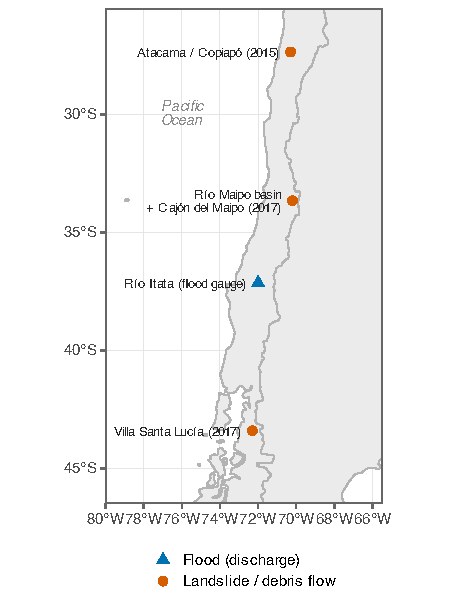
\includegraphics[width=0.48\linewidth]{figs/fig1_studyarea.pdf}
\caption{Sitios de estudio en Chile, del norte árido al sur húmedo. Naranjo:
sitios de deslizamientos/flujos de detritos, el backtest de deslizamientos del Río
Maipo, que además alberga el evento del Cajón del Maipo del 25 de febrero de 2017,
el evento de Atacama/Copiapó del 25 de marzo de 2015 y el evento de Villa Santa
Lucía del 16 de diciembre de 2017. Azul: la cuenca de validación de crecidas del
Río Itata (estación CAMELS-CL 8123001).}
\label{fig:studyarea}
\end{figure}

\section{Métodos}

\subsection{Métricas de backtesting}

La validación de un nowcast es verificación de pronóstico binario, lo que da una
tabla de contingencia $2\times2$ y los puntajes categóricos estándar: probabilidad
de detección (POD), razón de falsas alarmas (FAR), índice crítico de éxito (CSI) y
sesgo de frecuencia. Como el inventario está fechado solo a $\sim$mes, la unidad de
emparejamiento es el mes calendario, y el emparejamiento es \emph{event-céntrico}
con una ventana de tolerancia $\pm$ (un evento es acierto si una alerta cae dentro
de la ventana; una falsa alarma es un mes alertado lejos de cualquier evento) para
evitar inflar los fallos cuando un evento abarca una ventana de tolerancia. Para la
verificación \emph{espacial}, el emparejamiento por celda y mes contra un
inventario espacialmente disperso e \emph{incompleto} vuelve a CSI/FAR carentes de
sentido: casi toda ``falsa alarma'' es una celda susceptible y húmeda sin evento
\emph{registrado}. Puntuamos por tanto la discriminación, como hacen las
literaturas de susceptibilidad y de alerta temprana \citep{reichenbach2018}:
ROC-AUC \citep{hanley1982} (¿ordena el peligro las celdas-mes de evento por encima
de las tranquilas?) y POD a una fracción fija de área alertada. La incertidumbre
sobre el AUC se estima con un bootstrap de \emph{bloques mensuales} (remuestreando
meses calendario con reemplazo, manteniendo juntas las celdas de cada mes) de modo
que la autocorrelación espacial dentro del mes, la estructura dominante cuando una
tormenta moja muchas celdas, no se confunda con información independiente. Como
chequeo agnóstico al modelo, también entrenamos líneas base supervisadas (regresión
logística y gradient boosting \citep{friedman2001}) sobre atributos de
susceptibilidad y lluvia por celda-mes, evaluadas por validación cruzada
\texttt{GroupKFold} bloqueada por año, elegida por sobre una partición aleatoria
simple para evitar filtrar autocorrelación espacial intra-anual entre pliegues
\citep{roberts2016}.

Distinguimos dos nociones usadas a lo largo de los resultados. El
\emph{gatillado} pregunta si la forzante puede siquiera cruzar la curva I--D; es
una propiedad de la intensidad a la duración más fina resoluble, y un producto
diario puede fallarlo estructuralmente (Sección~5.4). La \emph{discriminación} (o
skill) hace la pregunta más difícil de si el peligro resultante \emph{ordena} las
ubicaciones de evento por encima de las de no evento, que es lo que miden ROC-AUC y
POD. Las dos no son intercambiables: una forzante puede gatillar con frecuencia y
aun así discriminar mal. El backtest distribuido (Sección~5.2) prueba la
discriminación sobre datos reales pero fechados a mes; un experimento sintético
controlado (Sección~5.3) la prueba bajo verdad de terreno conocida; el head-to-head
(Sección~5.4) aísla el gatillado.

\subsection{Calibración del umbral y validación por partición}

El intercepto I--D $a$ se calibra barriéndolo (con $b=0.39$ fijo) y seleccionando el
valor que maximiza el CSI contra los eventos fechados; $k=4$ y una ventana móvil
máxima de 7\,días (duraciones I--D de tormenta, no acumulación estacional) quedan
fijos. La pendiente $k$ entra solo a través del factor de gatillo
(Ec.~\ref{eq:logistic}), que es monótono en la excedencia, de modo que los puntajes
de discriminación basados en rangos (ROC-AUC, POD a área fija) son
\emph{exactamente} invariantes a $k$ para la configuración de solo gatillo, donde
el peligro es una función monótona de la excedencia; $k$ entra en los POD/FAR
basados en umbral solo a través del nivel de alerta elegido. La validación es por
partición: el intercepto se calibra en años calendario impares y se evalúa en años
pares.

\section{Resultados}

\subsection{Backtest agrupado de deslizamientos (Río Maipo)}
\label{sec:lumped}

Sobre 13\,880 pasos diarios (1979--2016) y 157 eventos fechados gatillados por
lluvia, el umbral global de Caine ($a=14.82$) se cruza en solo \textbf{7 de
13\,880 días} con forzante diaria CR2MET (POD $=0$): a 24\,h de duración la curva queda en $I_{\mathrm{crit}}=4.29$\,mm\,h$^{-1}$, un
total diario de 103\,mm, que solo esos siete días alcanzan, y ninguno cae en un mes
con evento. Un
intercepto regional $a^\star\approx5.5$\,mm\,h$^{-1}$ maximiza el CSI tanto en el
período completo como en los años impares, y la validación en años pares da POD
$\approx 0.50$ (Fig.~\ref{fig:idsweep}); pero el objetivo es plano (CSI 0.06--0.08
en $a=2$--13\,mm\,h$^{-1}$), así que $a^\star$ está débilmente identificado, y los
puntajes llevan intervalos anchos sobre los 19 meses con evento del registro: a
$\pm1$ mes, POD 0.53 [0.32, 0.73] y FAR 0.92 [0.85, 0.95] (Wilson 95\,\%). La
razón de falsas alarmas es estructural: con una tasa base de eventos cercana al
4\,\% de los meses y un único pluviómetro representativo en un clima mediterráneo
de estación húmeda, un gatillo I--D por sí solo sobre-predice (126 meses con
alerta, 28\,\% del registro). Si discrimina más allá de la estacionalidad es la
pregunta difícil, y la respuesta es marginal. Contra un nulo por barajado de años
que conserva la estacionalidad y el agrupamiento intra-anual de los meses con
alerta pero los reasigna a años aleatorios (2\,000 permutaciones), el CSI observado
de 0.077 se supera en el 10.5\,\% de las permutaciones (POD medio del nulo 0.46,
percentil 95 0.58), y un alertador que dispara todos los meses de mayo a
septiembre alcanza POD 0.47 con la misma tolerancia. El fechado a nivel de mes del
inventario sigue topando lo que cualquier gatillo puede puntuar aquí, pero la
subida del POD con la tolerancia de emparejamiento ($0.21\to0.68$ de $\pm0$ a
$\pm3$ meses, Tabla~\ref{tab:lumped}) no es evidencia de ello: el nulo sube igual
($0.27\to0.68$), igual que un alertador independiente a la misma tasa mensual
($0.28\to0.90$). El backtest agrupado muestra, por tanto, que $a^\star$ dispara el
gatillo en la estación correcta, no que separe los meses con evento del resto de la
estación húmeda; esa es la pregunta de discriminación que retoman el backtest
distribuido y el experimento controlado.

\begin{table}[ht]
\centering
\caption{Backtest agrupado del Maipo (contingencia mensual, emparejamiento $\pm1$ mes salvo indicación).}
\label{tab:lumped}
\resizebox{\linewidth}{!}{%
\begin{tabular}{@{}lccl@{}}
\toprule
Configuración & POD & FAR & nota \\
\midrule
Caine global, $a=14.82$ & 0.00 & 1.00 & dispara 7/13\,880 d, ninguno en mes de evento \\
Regional $a^\star=5.5$ (período completo) & 0.53 [0.32, 0.73] & 0.92 [0.85, 0.95] & calibración max-CSI; 19 meses con evento, Wilson 95\,\% \\
Regional $a^\star=5.5$ (partición) & 0.50 & 0.93 & calibra impares $\to$ valida pares \\
$a^\star=5.5$, tol. $\pm0/\pm1/\pm2/\pm3$\,meses & \multicolumn{2}{c}{POD 0.21/0.53/0.58/0.68} & sube como los nulos de abajo \\
Nulo por barajado de años, $\pm0/\pm1/\pm2/\pm3$\,meses & \multicolumn{2}{c}{POD 0.27/0.46/0.56/0.68 (media)} & 2\,000 perm.; $P(\mathrm{CSI}\geq0.077)=0.105$ a $\pm1$ \\
Alertador de estación húmeda (may--sep), $\pm1$\,mes & 0.47 & 0.95 & 190 meses con alerta, sin lluvia \\
\bottomrule
\end{tabular}}

\end{table}

\begin{figure}[t]
\centering
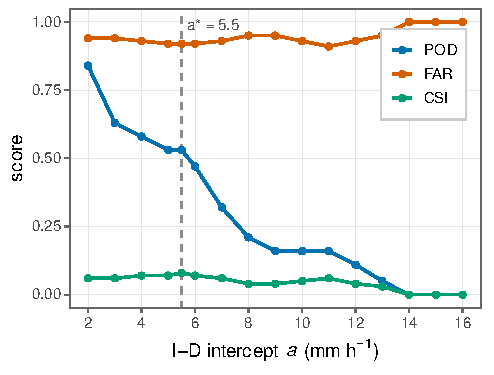
\includegraphics[width=0.62\linewidth]{figs/fig2_idsweep.pdf}
\caption{Calibración del intercepto I--D $a$ sobre el backtest agrupado del Maipo
(contingencia mensual, emparejamiento $\pm1$ mes). El POD cae y la razón de falsas
alarmas se mantiene alta a lo largo del barrido; el índice crítico de éxito es plano (0.06--0.08 en $a=2$--13\,mm\,h$^{-1}$) con su máximo en $a^\star\approx5.5$\,mm\,h$^{-1}$ (línea segmentada), muy por debajo
del valor global de Caine de 14.82: el intercepto queda débilmente identificado por este objetivo (Sección~\ref{sec:lumped}).}
\label{fig:idsweep}
\end{figure}

\paragraph{Los umbrales publicados no rescatan a la forzante diaria}
La auto-calibración invita a la objeción de que un umbral publicado, tomado tal
cual, podría hacerlo mejor. Lo probamos directamente aplicando, sin modificar, las
35 leyes de potencia I--D empíricas ($I=a\,D^{-b}$, mm\,h$^{-1}$) compiladas por
\citet{guzzetti2007} (las leyes de potencia puras de su Tabla~2, sin sus formas asintóticas ni
normalizadas) a la
misma forzante diaria CR2MET. El desenlace lo dicta la resolución, no la curva: 10
de las 35 quedan \emph{estructuralmente} por encima del techo diario --- en una
cuenca cuyo día más lluvioso en 38 años es 136\,mm, ninguna forzante diaria puede
alcanzar su intensidad de 24\,h, dado que la máxima intensidad de 24\,h resoluble
es el total diario dividido por 24 --- y 5 no disparan nunca. Trece dan POD $=0$, y
de las curvas que sí disparan, 30 tienen FAR $\geq 0.90$. La curva publicada con
mejor puntaje alcanza CSI $=0.084$, indistinguible del intercepto regional
auto-calibrado (CSI $=0.077$): el ensemble entero queda clavado cerca del mismo
punto de operación bajo. Una curva lo bastante alta como para ser selectiva queda
por encima del día más lluvioso (POD $0$); bajada lo suficiente para disparar,
dispara en la mayoría de los meses húmedos (FAR $\to 1$). La restricción
vinculante es la resolución de la forzante, no la elección del umbral publicado
(ejemplo \texttt{published\_thresholds}). Las mismas 35 curvas se reutilizan en la
Sección~\ref{sec:intercept} para mostrar que los resultados sub-diarios tampoco
dependen de la elección de curva.

\subsection{Backtest distribuido diario, un resultado nulo honesto}

Repitiendo el backtest con lluvia CR2MET \emph{distribuida} sobre una grilla
$15\times18$ (270 celdas, 123\,120 celdas-mes, 884 en la huella de eventos: la celda
de cada evento y las ocho que la rodean, en el mes del evento y los dos adyacentes, lo
que ubica los 157 eventos en 129 celdas), la
susceptibilidad RandomForest \emph{real} agregada a esa grilla por promedio de área, y verificación
espacial, se obtiene esencialmente \textbf{ninguna discriminación}
(Tabla~\ref{tab:auc}): el ROC-AUC es 0.463 para una línea base agrupada de media de
cuenca ponderada por susceptibilidad, 0.477 para lluvia distribuida con
susceptibilidad uniforme, y 0.485 para lluvia distribuida ponderada por
susceptibilidad real. Un bootstrap de bloques mensuales (remuestreando meses con
reemplazo, de modo que se preserva la autocorrelación espacial dentro del mes;
$B=2000$) sitúa los tres intervalos de confianza al 95\,\% cruzando el 0.5 del azar
($[0.40, 0.57]$ para la mejor configuración), y la probabilidad bootstrap de que el
AUC supere 0.5 es de solo 0.21--0.34. Ninguna de las configuraciones es
distinguible del azar. La lluvia media de 7 días en las celdas-mes con evento
registrado (39\,mm) es de hecho \emph{menor} que el promedio de la grilla (49\,mm).

\paragraph{De qué acusa este resultado nulo, y de qué no}
Ese último número merece escrutinio y no una mención al pasar: si los eventos
registrados caen donde llovió \emph{menos}, el dedo apunta al inventario o al campo
de lluvia, no al paso de tiempo, y sería interesado leerlo como evidencia de un
argumento de resolución. Probamos por tanto las explicaciones competidoras sobre
los mismos datos (ejemplo \texttt{null\_diagnosis}). \emph{¿Es una celda seca o un
mes seco?} Quitar el gradiente espacial estandarizando cada celda contra su propia
historia deja el nulo intacto (AUC 0.472; la anomalía media del mes de evento es
$z=-0.13$), así que no hay señal temporal enmascarada por la dimensión espacial.
\emph{¿Está el registro meramente desplazado?} Dilatar la \emph{etiqueta} ---
contando una celda-mes como positiva si hay un evento registrado dentro de $\pm k$
meses y $r$ celdas --- eleva el AUC solo a 0.496 con $\pm2$ meses y una celda de
holgura, todavía indistinguible del azar, así que los eventos no están simplemente
mal archivados por un mes o una celda. \emph{¿Es sesgo de exposición?} Las celdas
que alguna vez registran un evento reciben esencialmente la misma lluvia
climatológica que el resto ($-0.2$\,\%), aunque son levemente más susceptibles
(0.351 vs 0.329), así que el inventario no está concentrado en una parte
sistemáticamente más seca de la cuenca. De la forma más directa: una celda-mes con
evento registrado cae en el percentil 46 de la historia de su propia celda y en el
percentil 45 de la distribución espacial de su propio mes: en ambos ejes está donde
el azar la pondría.

La conclusión honesta es más fuerte y más estrecha que aquella que a este nulo se
le suele pedir sostener. El campo diario de 5\,km no lleva información recuperable
sobre dónde y cuándo fueron registrados estos eventos, y ninguna relajación
razonable de la etiqueta recupera alguna; pero eso es una afirmación sobre
\emph{este objetivo y este producto conjuntamente}, y no puede atribuirse a la
resolución temporal por sí sola. La evidencia para la afirmación sobre resolución
viene en cambio del experimento controlado, donde las etiquetas las genera un
proceso conocido (Sección~\ref{sec:synthetic}), y de la descomposición de campo por
factor único (Sección~\ref{sec:singlefactor}). Reportamos el nulo distribuido
porque un paper de método debe mostrar dónde su instrumento no lee nada, no porque
pruebe la tesis.

\begin{table}[ht]
\centering
\caption{Discriminación del backtest distribuido (ROC-AUC) con intervalos de
confianza al 95\,\% por bootstrap de bloques mensuales ($B=2000$). Todos los
intervalos cruzan 0.5.}
\label{tab:auc}
\begin{tabular}{@{}lccc@{}}
\toprule
configuración & AUC & IC 95\,\% & $P(\mathrm{AUC}>0.5)$ \\
\midrule
agrupada (media de cuenca) $\times$ susc. & 0.463 & $[0.375, 0.550]$ & 0.21 \\
distribuida, susc.\ $=1$           & 0.477 & $[0.399, 0.560]$ & 0.30 \\
distribuida $\times$ susc.\ real    & 0.485 & $[0.403, 0.565]$ & 0.34 \\
\bottomrule
\end{tabular}
\end{table}

Una línea base supervisada confirma que esto es una propiedad de los datos y no de
nuestro gatillo. Regresión logística y gradient boosting entrenados sobre atributos
por celda-mes (susceptibilidad; total mensual; lluvia máxima de 1 día y de 7 días;
total del mes anterior), evaluados con \texttt{GroupKFold} bloqueado por año,
alcanzan un AUC de validación cruzada de solo 0.56 y 0.52, apenas por encima del
azar. Un análisis de atributo único ubica la poca señal que existe: viene de la
susceptibilidad estática (AUC 0.55, ella misma una cota superior optimista dado que
este ráster fue entrenado sobre el mismo inventario, Sección~3) y de una débil
humedad antecedente (0.52), mientras que todo atributo de intensidad de lluvia está
en o por debajo del azar (máx 7 días 0.49, máx 1 día 0.46, total mensual 0.46). La
lluvia diaria no lleva por tanto esencialmente ninguna información sobre dónde y
cuándo ocurrieron estos deslizamientos, y un modelo flexible no puede recuperar una
señal que el producto diario no contiene. El 0.485 de nuestro motor incluso cae
levemente por debajo de la susceptibilidad sola, porque multiplicar la
susceptibilidad por un factor de lluvia diaria casi aleatorio la diluye: a esta
resolución el gatillo diario es peor que ninguno.

\begin{figure}[t]
\centering
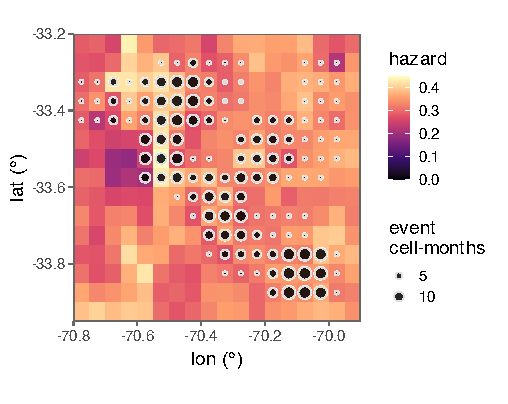
\includegraphics[width=0.6\linewidth]{figs/fig4_hazard.pdf}
\caption{Ejemplo de campo de peligro distribuido sobre la región de eventos del Río
Maipo (grilla CR2MET 15$\times$18) en el paso más lluvioso, con susceptibilidad
RandomForest real y el gatillo I--D regional ($a=5.5$); los puntos marcan las celdas
de la huella del inventario, con tamaño según su número de celdas-mes con evento
registrado (884 en 129 celdas). Ninguna celda alcanza el nivel de alerta 0.5 en este paso. El campo está
espacialmente estructurado y, sin embargo, a resolución diaria de 5\,km no separa
las celdas-mes con evento registrado (Sección~5.2); la Fig.~\ref{fig:synthetic}
muestra, sobre datos controlados, cómo esa discriminación vuelve al aumentar la
resolución.}
\label{fig:hazard}
\end{figure}

\subsection{Experimento controlado de resolución}
\label{sec:synthetic}

El nulo distribuido es ambiguo por sí solo: un AUC casi aleatorio podría significar
que el motor no tiene skill, o que el inventario incompleto y fechado a mes no
puede revelar el skill que sí está presente. Resolvemos la ambigüedad con un
experimento controlado cuya verdad de terreno es conocida.

\paragraph{Las etiquetas no vienen de la regla bajo prueba}
Un experimento sintético que define un evento como ``una ráfaga que cruza la curva
I--D'' y luego reporta que un gatillo I--D la recupera es deductivo: el resultado
está implicado por la construcción, no es evidencia sobre ella. Generamos por tanto
las etiquetas con un mecanismo de falla \emph{independiente}. Sobre una grilla
$20\times20$ durante 60 días sintetizamos un campo de lluvia semihorario con dos
tipos de día --- una ráfaga de ${\sim}1$\,h (8--30\,mm) y un total similar o mayor
(16--46\,mm) repartido entre 8 y 23\,h --- y luego decidimos la falla con un
análogo de presión de poros transitoria: un almacenamiento lineal alimentado por
infiltración con tope (el exceso escurre) y drenado con una constante de tiempo de
${\sim}4$\,h, que falla la celda-día cuando supera
$\theta_\mathrm{crit}=12$\,mm. Esta es una forma funcional distinta de
$I=a\,D^{-b}$, y las dos no coinciden: por realización cerca de 123 de 667 ráfagas
nunca fallan, y cerca de 1167 fallas caen en días que \emph{no} fueron ráfagas, de
modo que la etiqueta no es un renombre del tipo de día. De forma crítica, el
almacenamiento se integra siempre al paso nativo semihorario --- la física ocurre a
resolución completa y lo que degradamos es la \emph{observación}. La
susceptibilidad está estructurada pero no correlacionada con qué días fallan, así
que no lleva información separadora. Luego agregamos el campo idéntico de 0.5\,h a
24\,h, manteniendo fijos el motor y la duración máxima de 24\,h, y puntuamos contra
las etiquetas físicas sobre 20 realizaciones aleatorias
(Fig.~\ref{fig:synthetic}).

\paragraph{La agregación destruye una ruta de falla y respeta la otra}
El almacenamiento falla celdas-día por dos caminos: una ráfaga que le gana al
drenaje, y lluvia más lenta que se acumula más allá de $\theta_\mathrm{crit}$. La
agregación no los trata igual, y ese es el resultado. \textbf{Estratificada por
mecanismo, la tasa operacional de captura de las fallas por ráfaga colapsa de
$0.46\pm0.09$ en semihorario a $0.00\pm0.01$ en diario, mientras que las fallas por
acumulación se capturan en ${\approx}0.42$ a \emph{toda} resolución} (POD con un
presupuesto de área alertada del 5\,\%). El colapso mismo es esperable por el diseño y no lo presentamos como un descubrimiento: ninguna ráfaga del rango 8--30\,mm supera la curva de $a^\star$ una vez repartida en 24\,h (la mayor da $E=0.79$; cruzar el techo diario con $a^\star=5.5$ requiere 38\,mm en un día), así que lo que el experimento mide es dónde, entre lo semihorario y lo diario, cae la tasa de captura, y que las fallas por acumulación quedan a salvo, no si la forzante diaria puede alguna vez ver una ráfaga. Las ráfagas lo bastante grandes para cruzar el techo diario son los 7 días del Maipo de la Sección~\ref{sec:lumped}. Mover las perillas del diseño una a la vez (Tabla~\ref{tab:sweep}; cinco realizaciones cada una) dice dónde vive el colapso. Es una propiedad de la magnitud de la ráfaga relativa al techo diario: con ráfagas de 30--60\,mm, a caballo del techo, la tasa de captura diaria de las fallas por ráfaga se queda en 0.46, y con ráfagas de 60--120\,mm el producto diario puntúa \emph{más alto} que el semihorario (0.70 contra 0.47), porque una ráfaga que domina su día es más fácil de ordenar en el paso grueso. La constante de tiempo de drenaje decide otra cosa: con $\tau$ de 24 o 120\,h las fallas pasan a estar controladas por la humedad antecedente y el gatillo I--D captura menos del 10\,\% de las fallas por acumulación a \emph{cualquier} resolución (0.09 y 0.04 a semihorario), lo que es un límite del gatillo, no de la forzante; ese caso se retoma en la Sección~\ref{sec:limits}. La humedad de falla $\theta_\mathrm{crit}$ mueve la mezcla de las dos rutas (a 24\,mm no ocurren fallas por acumulación; a 6\,mm dominan) sin cambiar la forma del colapso por ráfaga, y el intercepto global de Caine corre el techo a 103\,mm por día y deja el colapso en su lugar. La regla de estratificación es la clase generadora: una falla es por ráfaga si su celda-día se generó como ráfaga, por acumulación en otro caso; las semillas son deterministas (paso de razón áurea desde una base fija) y el ejemplo las imprime.

\begin{table}[ht]
\centering
\small
\caption{Barrido uno a la vez del experimento controlado (cinco realizaciones por fila): POD con presupuesto de área alertada del 5\,\% sobre fallas por ráfaga a resolución semihoraria y diaria, la resolución más gruesa a la que sigue siendo al menos la mitad de su valor semihorario, y POD sobre fallas por acumulación. ``Techo'' es el total diario con el que una ráfaga repartida en 24\,h alcanza la curva, $a\cdot24^{1-b}$.}
\label{tab:sweep}
\resizebox{\linewidth}{!}{%
\begin{tabular}{@{}lcccc@{}}
\toprule
Configuración & Techo (mm) & POD ráfaga 0.5\,h $\to$ 24\,h & Resolución de medio POD & POD acum.\ 0.5\,h $\to$ 24\,h \\
\midrule
Paper: ráfagas 8--30\,mm, $\tau$ 4\,h, $\theta$ 12\,mm, $a^\star$ 5.5 & 38 & 0.49 $\to$ 0.00 & 6\,h & 0.45 $\to$ 0.43 \\
Ráfagas 30--60\,mm & 38 & 0.48 $\to$ 0.46 & 24\,h & 0.40 $\to$ 0.33 \\
Ráfagas 60--120\,mm & 38 & 0.47 $\to$ 0.70 & 24\,h & 0.38 $\to$ 0.28 \\
$\tau$ 1\,h & 38 & 0.49 $\to$ 0.00 & 6\,h & sin fallas por acumulación \\
$\tau$ 24\,h & 38 & 0.49 $\to$ 0.00 & 3\,h & 0.09 $\to$ 0.12 \\
$\tau$ 120\,h & 38 & 0.49 $\to$ 0.00 & 3\,h & 0.04 $\to$ 0.05 \\
$\theta_\mathrm{crit}$ 6\,mm & 38 & 0.49 $\to$ 0.00 & 3\,h & 0.16 $\to$ 0.23 \\
$\theta_\mathrm{crit}$ 24\,mm & 38 & 0.50 $\to$ 0.00 & 12\,h & sin fallas por acumulación \\
Caine, $a=14.82$ & 103 & 0.98 $\to$ 0.00 & 3\,h & 0.44 $\to$ 0.43 \\
Ráfagas 60--120\,mm, $a=14.82$ & 103 & 0.96 $\to$ 0.96 & 24\,h & 0.10 $\to$ 0.22 \\
\bottomrule
\end{tabular}}

\end{table} La tasa de gatillado cae del 27\,\% al
9\,\% de las celdas-día en el mismo barrido.

Los puntajes agrupados, en cambio, decaen solo levemente --- AUC de solo gatillo
$0.99\to0.92$, ponderado por susceptibilidad $0.93\to0.91$, POD@5\,\% agrupado
$0.43\to0.29$ --- y esa levedad es en sí misma informativa: el número agrupado
promedia una población que la agregación aniquila con otra que deja intacta, de
modo que reportarlo solo escondería el efecto por completo. Con estas etiquetas, el
68\,\% de las fallas son por acumulación, y esas un producto diario las captura
perfectamente bien. La afirmación honesta no es entonces que la forzante diaria sea
ciega, sino que es ciega \emph{a la ruta de gatillado sub-diaria} --- que es la ruta
que un nowcast I--D existe para atrapar, y la que los casos de campo confirman
(Sección~\ref{sec:singlefactor}, donde la resolución voltea la detección solo para
la ráfaga breve del Cajón del Maipo). El experimento aísla el \emph{mecanismo de
agregación} bajo verdad de terreno conocida con el modelo y el terreno fijos; no es
una afirmación sobre tasas base de eventos reales, de lo que se ocupan los
backtests de campo (Secciones~5.1--5.2).

\begin{figure}[t]
\centering
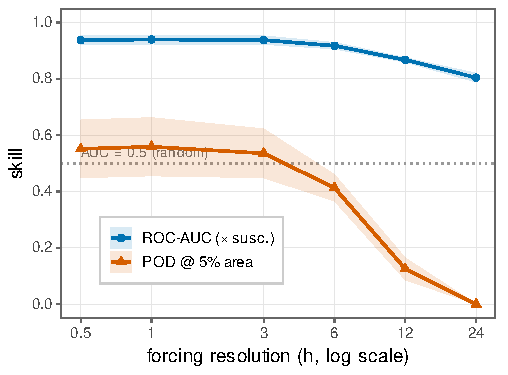
\includegraphics[width=0.6\linewidth]{figs/fig_synthetic.pdf}
\caption{Experimento controlado de resolución (media sobre 20 realizaciones
aleatorias; bandas $\pm1$ de). Campos de lluvia sintéticos semihorarios, agregados
a resolución más gruesa (eje logarítmico) bajo un motor I--D fijo (regional
calibrado $a^\star=5.5$) y duración máxima de 24\,h, puntuados contra etiquetas
provenientes de un almacenamiento de presión de poros \emph{independiente} y no de
la regla I--D misma. Estratificar por mecanismo de falla es lo que revela el
efecto: la tasa operacional de captura de las fallas \textbf{por ráfaga} (naranjo)
colapsa de 0.46 a 0.00, mientras que las fallas \textbf{por acumulación} (verde) se
capturan en ${\approx}0.42$ a toda resolución. El AUC agrupado ponderado por
susceptibilidad (azul) apenas se mueve ($0.93\to0.91$) precisamente porque promedia
ambas, y por eso un puntaje agrupado esconde el fenómeno. La agregación diaria
(intensidad topada en total$/24$\,h) destruye específicamente la ruta de gatillado
sub-diaria, con el modelo y el terreno fijos.}
\label{fig:synthetic}
\end{figure}

\subsection{Head-to-head de resolución}
\label{sec:headtohead}

El nulo anterior motiva una comparación controlada de la resolución de la forzante
sobre el mismo núcleo de tormenta (Atacama, 24--26 de marzo de 2015; el máximo del
total del evento en IMERG en lon $-70.45$, lat $-27.15$), con el motor I--D
idéntico (Tabla~\ref{tab:headtohead}). El núcleo se selecciona
\emph{condicionalmente al evento conocido}, así que esta es una comparación de
gatillado y timing --- si cada producto puede cruzar la curva, y cuándo --- no una
prueba de discriminación; la discriminación es asunto del backtest distribuido
(Sección~5.2) y del experimento controlado (Sección~\ref{sec:synthetic}). A lo
largo de esta sección y la siguiente usamos el intercepto regional
$a^\star=5.5$\,mm\,h$^{-1}$ calibrado en la Sección~\ref{sec:lumped} --- la única
curva I--D ajustada a datos en este trabajo --- en vez de un valor elegido para que
la comparación funcione; la Sección~\ref{sec:intercept} muestra que la conclusión
no descansa en esa elección. Con un valor diario la duración más fina resoluble es
24\,h, de modo que la máxima intensidad media resoluble es (total diario)$/24$\,h:
CR2MET ve 30.1\,mm repartidos en 0.66\,mm\,h$^{-1}$, una excedencia de a lo más
0.45 (con el regional calibrado $a^\star=5.5$) o 0.17 (Caine); el producto diario
\textbf{estructuralmente no puede gatillar} para la profundidad diaria de esta
tormenta (su día más lluvioso es 15.9\,mm); un total diario mayor sí cruza la
curva, como muestran los 7 días del Maipo de la Sección~\ref{sec:lumped}. El mismo
núcleo de tormenta en IMERG semihorario alcanza un peak de 40\,mm\,h$^{-1}$; el
umbral I--D se cruza a las 04:30 UTC del 24 de marzo ($E\approx9$), horas antes de
los flujos documentados (Fig.~\ref{fig:leadtime}). Una forzante de mayor resolución
supera el límite sin cambio alguno en el motor.

Esta comparación, sin embargo, mueve \emph{dos} cosas a la vez. Los dos productos
también difieren en magnitud (IMERG 108\,mm vs CR2MET 30\,mm en este núcleo); se
sabe que IMERG sobreestima en regímenes convectivos áridos mientras que CR2MET,
mezclado con pluviómetros sobre una zona casi sin estaciones, probablemente
subestima, de modo que el total verdadero queda en medio. Un contraste
CR2MET-diario vs IMERG-semihorario confunde por tanto el producto con su
resolución, y la Sección~\ref{sec:singlefactor} los separa explícitamente --- con
un resultado que matiza a este, ya que en \emph{este} evento es el producto, no la
resolución, lo que decide la detección. Lo que sobrevive intacto a la separación es
el timing: ningún producto diario, cualquiera sea su magnitud, puede situar el
cruce a las 04:30. La parte puramente aritmética del argumento es además
independiente de la disputa de magnitud: incluso tomando el propio total de 30\,mm
de CR2MET, repartirlo en 24\,h da una intensidad media muy por debajo de la curva
I--D, así que un producto diario no puede gatillar sin importar cuál magnitud sea
la correcta.

\begin{table}[ht]
\centering
\caption{CR2MET diario vs.\ GPM IMERG semihorario en el núcleo de tormenta de Atacama (mismo motor I--D).}
\label{tab:headtohead}
\resizebox{\linewidth}{!}{%
\begin{tabular}{@{}lcc@{}}
\toprule
 & CR2MET diario ($\sim$5\,km) & IMERG $\frac{1}{2}$-horario ($\sim$10\,km) \\
\midrule
total del evento (24--26 de marzo, celda núcleo) & 30.1\,mm & 108.5\,mm \\
día / media hora más lluviosos & 15.9\,mm & 20.0\,mm \\
duración más fina resoluble & 24\,h & 0.5\,h \\
máx. intensidad resoluble (paso más lluvioso$/$duración) & 0.66\,mm\,h$^{-1}$ & 40.0\,mm\,h$^{-1}$ \\
I--D ($a^\star=5.5$) & sin alerta ($E\leq0.45$) & alerta 24-mar 04:30 ($E\approx9$) \\
\bottomrule
\end{tabular}}

\end{table}

\begin{figure}[t]
\centering
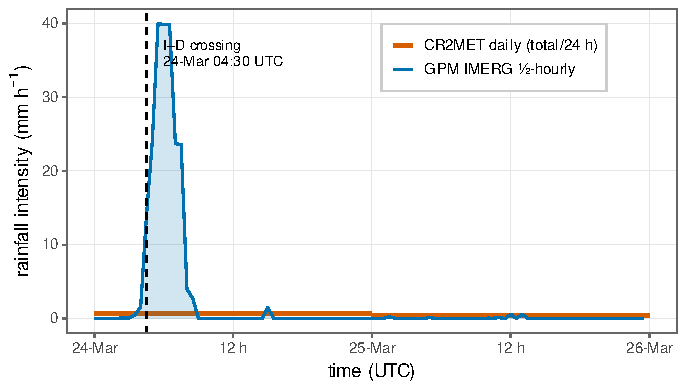
\includegraphics[width=0.78\linewidth]{figs/fig3_leadtime.pdf}
\caption{Resolución de la forzante en el núcleo de tormenta de Atacama (24--26 de
marzo de 2015). La intensidad semihoraria de GPM IMERG (azul) alcanza un peak de
40\,mm\,h$^{-1}$ y cruza la curva I--D a las 04:30 UTC del 24 de marzo; la misma
lluvia vista por un producto diario (CR2MET, naranjo: total$/24$\,h) es un valor
plano de 0.66\,mm\,h$^{-1}$ el día más lluvioso (y menor los demás) que nunca alcanza la curva. El producto diario
estructuralmente no puede resolver la ráfaga gatillante.}
\label{fig:leadtime}
\end{figure}

\subsection{Lead time sub-diario multi-evento}
\label{sec:multievent}

El resultado sub-diario se generaliza a tres eventos fechados de flujos de detritos
en climas opuestos (Tabla~\ref{tab:multievent}). En los tres, el cruce I--D
semihorario cae sobre el día documentado o justo antes. Para la ráfaga convectiva
de verano del Cajón del Maipo, la misma lluvia agregada a diaria \textbf{nunca
gatilla}, solo la resolución sub-diaria la detecta --- nótese que esta columna ya
mantiene fijo el producto, dado que agrega la misma serie IMERG, que es la
comparación que la Sección~\ref{sec:singlefactor} generaliza. El inventario no
entrega la \emph{hora} de inicio del evento, así que estos no son puntajes formales
de skill de lead time sino una demostración de que la forzante sub-diaria resuelve
el tiempo de cruce del umbral que la forzante diaria no puede.

Como chequeo espacial de falsas alarmas, corrimos el gatillo I--D idéntico por
celda sobre la escena IMERG completa de cada evento. El núcleo de tormenta
documentado es en todos los casos la celda más extrema (percentil 96.7--100 de
excedencia peak), pero el gatillo cruza la curva sobre una huella amplia: 30\,\% de
la escena de Atacama, 6\,\% en el Cajón del Maipo, y la totalidad del recuadro
(pequeño, frontal) de Villa Santa Lucía, de modo que el cruce no es espacialmente
disperso dentro de estas escenas centradas en la tormenta. Esto ubica el
\emph{peak} correctamente pero \emph{no} es una tasa baja de falsas alarmas, y como
el recuadro está centrado en el evento por construcción, es esperable una fracción
alta de cruce. Una estimación genuina de discriminación necesita la frecuencia de
cruce fuera de evento en estos núcleos, un registro sub-diario multi-anual en días
\emph{sin} un flujo documentado, que los gránulos de ventana de evento actuales no
proveen. Los resultados sub-diarios son por tanto demostraciones de gatillado y
timing, no puntajes de skill; ensamblar ese registro sub-diario multi-anual es,
junto con un inventario con resolución de día (Sección~7), el paso de validación
clave que queda pendiente.

\begin{table}[ht]
\centering
\caption{Cruce I--D sub-diario en tres eventos (GPM IMERG semihorario, núcleo de
tormenta, regional calibrado $a^\star=5.5$).}
\label{tab:multievent}
\resizebox{\linewidth}{!}{%
\begin{tabular}{@{}llcccc@{}}
\toprule
Evento & Clima & Total & Peak 1\,h & Cruce (UTC) & ¿Dispara el diario? \\
\midrule
Atacama/Copiapó & árido, convectivo & 108\,mm & 40\,mm\,h$^{-1}$ & 24-mar 04:30 & sí \\
Cajón del Maipo & Andes, verano & 28\,mm & 5\,mm\,h$^{-1}$ & 25-feb 17:30 & \textbf{no} \\
Villa Santa Lucía & húmedo, frontal & 83\,mm & 17\,mm\,h$^{-1}$ & 15-dic 15:30 & sí \\
\bottomrule
\end{tabular}}

\end{table}

\paragraph{Frente a un nowcast operacional}
El nowcast diario de LHASA versión 2 \citep{stanley2021,lhasa2023data}, la cadena
operacional con que más a menudo se compara el motor, está archivado del 3 de abril de
2015 al 10 de febrero de 2021, así que cubre los eventos del Cajón del Maipo y de Villa
Santa Lucía pero no el de Atacama. Leímos su probabilidad sobre el recuadro de cada
evento en los siete días alrededor del evento. En el recuadro del Cajón del Maipo el
percentil 99 sube de 0.25 el 20 de febrero a 0.65, 0.91 y 0.93 el 23--25 de febrero,
con un 13\,\% del recuadro en 0.3 o más el 25, el día en que el motor cruza a las 17:30
UTC; en la propia celda núcleo de IMERG, sin embargo, LHASA ya da 0.95 en los días
secos del 20--21 de febrero, así que su valor a nivel de celda no singulariza el día
del evento. En Villa Santa Lucía la probabilidad en el pueblo llega a 0.59 en el nowcast
fechado el 15 de diciembre (62\,\% del recuadro en 0.1 o más) y cae a 0.07 el 16; el motor
cruza el 15 de diciembre a las 15:30 UTC, y el flujo está fechado el 16 de diciembre.
Ambos sistemas marcan el mismo día; el motor agrega la hora, LHASA agrega el estado
antecedente y la susceptibilidad con que fue entrenado. Dos eventos y ninguna tasa
fuera de evento hacen de esto un chequeo de consistencia, no una comparación de skill.

\subsection{Separando el producto de su resolución}
\label{sec:singlefactor}

El head-to-head de la Sección~\ref{sec:headtohead} varía dos cosas a la vez. CR2MET
diario e IMERG semihorario difieren tanto en resolución temporal como en el
producto de lluvia mismo, y en estos núcleos de tormenta los dos productos difieren
hasta en un factor de cuatro en el total del evento. Atribuir toda la diferencia a
la resolución es por tanto poco sólido. Separamos los factores insertando la celda
faltante del diseño: la \emph{misma} serie IMERG agregada a 24\,h. Cada comparación
adyacente mueve entonces exactamente un factor,
\begin{center}
A. CR2MET diario $\;\xrightarrow{\text{producto}}\;$ B. IMERG agregado a 24\,h
$\;\xrightarrow{\text{resolución}}\;$ C. IMERG semihorario,
\end{center}
y como la excedencia es multiplicativa en la intensidad, la razón total factoriza
exactamente, $E_C/E_A = (E_B/E_A)\cdot(E_C/E_B)$. Para mantener conservadora la
prueba, CR2MET se lee como el \emph{máximo} sobre sus celdas dentro del píxel IMERG
(dándole al producto diario su mejor oportunidad frente a la tormenta), y las tres
configuraciones ven la misma ventana de evento y el mismo motor.

El desenlace (Tabla~\ref{tab:singlefactor}) es más discriminante de lo que el
head-to-head sugería, y revisa cómo debe leerse esa comparación. En Atacama el
factor de resolución es sustancial ($\times3.2$) pero el factor de \emph{producto}
es el doble de grande ($\times6.2$), y es el producto el que voltea la detección:
IMERG agregado a diario ya cruza la curva ($E=2.8$). La afirmación que sostiene el
caso sub-diario en este evento es entonces sobre timing, no sobre detección --- la
serie diaria marca el día, solo la semihoraria sitúa el cruce a las 04:30. En Villa
Santa Lucía ningún factor voltea nada: CR2MET diario ya gatilla ($E=1.6$), y la
resolución vuelve a comprar solo timing. Solo en el Cajón del Maipo la resolución
voltea la detección con el producto fijo ($E=0.45\to1.23$), y allí el factor de
producto no lo hace ($E=0.18\to0.45$, todavía bajo la curva).

Así que de tres eventos, la resolución cambia la \emph{detección} en uno, y en ese
la ráfaga es breve y débil --- precisamente el régimen que el argumento de
agregación predice. En los tres cambia el \emph{timing}, que ningún producto diario
puede entregar con ninguna magnitud. Enunciamos la distinción con claridad porque
las dos afirmaciones tienen fuerza distinta: la forzante sub-diaria entrega lead
time intra-diario en general, mientras que rescata la detección específicamente
para ráfagas breves, y un caso como Atacama, donde un producto diario con la
magnitud correcta habría disparado igual, no es evidencia de la segunda afirmación.
El experimento controlado de la Sección~\ref{sec:synthetic}, donde el producto está
fijo por construcción y solo varía la resolución, es lo que aísla el efecto de
detección a escala.

\begin{table}[ht]
\centering
\caption{Descomposición por factor único en cada núcleo de tormenta: el factor de
producto (A$\to$B) y el factor de resolución (B$\to$C) sobre la excedencia I--D
peak $E$ ($a^\star=5.5$). La negrita marca el paso que voltea la detección ($E$
cruzando 1). La fila de CR2MET (A) es el máximo sobre las celdas CR2MET dentro del
píxel IMERG en la ventana $D$ de la descomposición, así que su total (26.8\,mm en
Atacama) no es el total de tres días de la celda núcleo de la Tabla~\ref{tab:headtohead} (30.1\,mm).}
\label{tab:singlefactor}
\small
\resizebox{\linewidth}{!}{%
\begin{tabular}{@{}llccccc@{}}
\toprule
Evento & Configuración & Total & $I_{\max}$ & $D$ & $E$ & ¿Dispara? \\
 & & (mm) & (mm\,h$^{-1}$) & (h) & & \\
\midrule
\multirow{3}{*}{Atacama/Copiapó}
 & A. CR2MET diario        & 26.8 & 0.55 & 48 & 0.45 & no \\
 & B. IMERG a 24\,h        & 108.5 & 4.48 & 24 & \textbf{2.82} & \textbf{sí} \\
 & C. IMERG semihorario    & 108.5 & 31.81 & 3 & 8.88 & sí \\
\multicolumn{7}{@{}l}{\quad\emph{producto} $\times6.2$ $\cdot$ \emph{resolución} $\times3.2$ --- \emph{el producto voltea la detección; la resolución agrega timing}} \\
\midrule
\multirow{3}{*}{Cajón del Maipo}
 & A. CR2MET diario        & 6.9 & 0.29 & 24 & 0.18 & no \\
 & B. IMERG a 24\,h        & 27.5 & 0.54 & 48 & 0.45 & no \\
 & C. IMERG semihorario    & 27.5 & 4.41 & 3 & \textbf{1.23} & \textbf{sí} \\
\multicolumn{7}{@{}l}{\quad\emph{producto} $\times2.5$ $\cdot$ \emph{resolución} $\times2.8$ --- \emph{la resolución voltea la detección, el producto solo no}} \\
\midrule
\multirow{3}{*}{Villa Santa Lucía}
 & A. CR2MET diario        & 72.2 & 2.53 & 24 & 1.59 & sí \\
 & B. IMERG a 24\,h        & 83.1 & 2.73 & 24 & 1.72 & sí \\
 & C. IMERG semihorario    & 83.1 & 12.43 & 3 & 3.47 & sí \\
\multicolumn{7}{@{}l}{\quad\emph{producto} $\times1.1$ $\cdot$ \emph{resolución} $\times2.0$ --- \emph{ninguno voltea la detección; la resolución agrega timing}} \\
\bottomrule
\end{tabular}}

\end{table}

\subsection{El resultado sub-diario no descansa en el intercepto elegido}
\label{sec:intercept}

Las Secciones~\ref{sec:headtohead}--\ref{sec:multievent} aplican una sola curva
I--D, y un lector escéptico puede razonablemente preguntar si la conclusión es un
artefacto de esa elección: un intercepto lo bastante bajo hace gatillar cualquier
tormenta, y uno lo bastante alto no hace gatillar ninguna. Removemos la elección de
dos maneras.

Primero, el intercepto puede \emph{medirse} en vez de elegirse. Como la excedencia
escala exactamente como $1/a$ --- $E(a)=I\,D^{b}/a$, de modo que
$E(a)=(a_0/a)\,E(a_0)$ --- y la ventana que la maximiza es por tanto la misma para
todo $a$, cada evento tiene un \emph{intercepto crítico} bien definido
\begin{equation}
a_\mathrm{crit} \;=\; \max_{t,m}\; I(t,m)\,D(m)^{b},
\label{eq:acrit}
\end{equation}
el intercepto más alto con el que ese evento todavía cruza la curva. Es una
propiedad de la lluvia observada y de $b$, no del analista. Calcularlo sobre la
serie semihoraria y sobre la misma serie agregada a diaria da dos valores, y el
intervalo entre ellos,
$a_\mathrm{crit}(\text{diario}) < a \leq a_\mathrm{crit}(\text{semihorario})$, es la
banda de umbrales en la que la \emph{resolución por sí sola} decide la detección.
Esa banda abarca un factor de 2.0--3.2 en $a$ en los tres eventos
(Tabla~\ref{tab:intercept}), y el $a^\star=5.5$ calibrado cae dentro de ella en el
Cajón del Maipo --- que es la razón por la que el producto diario pierde ese evento
con el intercepto que el paper calibra de forma independiente, en el backtest del
Maipo, y no con uno afinado para esta comparación.

Segundo, y sin seleccionar intercepto alguno, volvimos a correr las 35 leyes de
potencia publicadas por \citet{guzzetti2007} --- cada una con su propio $(a,b)$,
sin modificar --- sobre cada evento en ambas resoluciones. La resolución voltea el
desenlace (dispara el sub-diario, no el diario) en 8 de 35 curvas en Atacama, 8 de
35 en Villa Santa Lucía y 2 de 35 en el Cajón del Maipo. La cifra del Cajón del
Maipo enuncia además el límite honesto de ese evento: es una ráfaga débil (28\,mm,
peak de 5\,mm\,h$^{-1}$) que solo 4 de las 35 curvas publicadas detectan a
\emph{cualquier} resolución, así que si bien el efecto de resolución allí es real,
está demostrado sobre un evento cercano al piso de detección de la literatura. En
los dos eventos más fuertes, donde la mayoría de las curvas publicadas sí dispara,
el efecto de resolución lo lleva aproximadamente un cuarto del ensemble. Ambos
análisis los reproduce el ejemplo \texttt{intercept\_sensitivity}.

Dos salvedades acotan esto. Aplicar $a^\star$, ajustado en el Río Maipo, a
tormentas en el Atacama y en Patagonia es una transferencia muy fuera de su región
de calibración, y no afirmamos que 5.5\,mm\,h$^{-1}$ sea la curva regional correcta
para ninguna de las dos; el punto de la Tabla~\ref{tab:intercept} es precisamente
que el resultado de resolución sobrevive a cualquier intercepto que se adopte
dentro de una banda amplia, así que no se necesita tal afirmación. Y $b$ se
mantiene en 0.39 en todo momento: el intercepto crítico de la Ec.~\ref{eq:acrit}
está definido para un exponente dado, y el ensemble de curvas publicadas, que varía
$b$ de 0.19 a 1.50, es lo que cubre esa dimensión.

\begin{table}[ht]
\centering
\caption{Intercepto I--D crítico $a_\mathrm{crit}$ (Ec.~\ref{eq:acrit}, $b=0.39$)
por evento y resolución de la forzante, y la banda de interceptos en la que la
resolución por sí sola decide la detección.}
\label{tab:intercept}
\resizebox{\linewidth}{!}{%
\begin{tabular}{@{}lcccc@{}}
\toprule
Evento & $a_\mathrm{crit}$ semihorario & $a_\mathrm{crit}$ diario & razón & la resolución decide para \\
 & (mm\,h$^{-1}$) & (mm\,h$^{-1}$) & & (mm\,h$^{-1}$) \\
\midrule
Atacama/Copiapó & 48.8 & 15.5 & 3.2$\times$ & $15.5 < a \leq 48.8$ \\
Cajón del Maipo & 6.8 & 2.5 & 2.8$\times$ & $2.5 < a \leq 6.8$ \hfill ($\ni a^\star$) \\
Villa Santa Lucía & 19.1 & 9.4 & 2.0$\times$ & $9.4 < a \leq 19.1$ \\
\bottomrule
\end{tabular}}

\end{table}

\paragraph{Sensibilidad a los demás hiperparámetros}
El exponente $b$, la duración máxima I--D, la pendiente logística $k$ y el nivel de alerta se mantienen fijos en el resto del paper. Mover cada uno a la vez sobre el backtest agrupado (Tabla~\ref{tab:oat}) muestra que el \emph{óptimo} se mueve y el \emph{skill en el óptimo} no: recalibrar $a^\star$ por CSI máximo con $b=0.19$, $0.565$ (la mediana de las 35 curvas publicadas) y $0.78$ da $a^\star$ de 2.5, 13.5 y 13.0\,mm\,h$^{-1}$ con CSI 0.080, 0.082 y 0.066 contra 0.077 en la configuración del paper, y cada par (pendiente, nivel), que entra solo por la excedencia a la que el peligro cruza el nivel, $E_\mathrm{thr}=1+\ln[L/(1-L)]/k$, deja el CSI entre 0.071 y 0.079. Con el $a^\star=5.5$ fijo del paper los puntajes sí se mueven con $b$ (POD 0.11 con $b=0.19$, 0.89 con $b=0.78$), que es la afirmación de que $a$ y $b$ no están identificados por separado por una contingencia mensual. En los tres núcleos de tormenta la excedencia semihoraria cambia poco con $b$ pero la diaria cambia mucho, porque la ventana diaria es de 24\,h y $D^b$ crece con $b$: con $b=0.78$ la serie diaria de Atacama y de Villa Santa Lucía cruza con holgura y el valor diario del Cajón del Maipo llega a 1.47, así que la columna ``lo diario no dispara'' de la Tabla~\ref{tab:singlefactor} es la sensible a $b$ y se sostiene para exponentes hasta cerca de 0.6. Los puntajes por rango son invariantes a $k$ por construcción (Sección~4.2) y no se volvieron a correr; el operador de agregación de 30\,m a 5\,km de la Sección~5.2 (el promedio de área) no se varió, lo que sigue siendo un vacío.

\begin{table}[ht]
\centering
\small
\caption{Sensibilidad uno a la vez del backtest agrupado del Maipo ($\pm1$ mes) y de las excedencias de los núcleos de tormenta. Izquierda: el intercepto de CSI máximo recalibrado bajo cada configuración, con POD/FAR/CSI en ese óptimo y en el $a^\star=5.5$ fijo del paper. Derecha: excedencia peak $E$ con $a^\star=5.5$ para la serie semihoraria y la diaria de cada núcleo (ventana máxima de 24\,h), que cruza la curva cuando $E\geq1$.}
\label{tab:oat}
\resizebox{\linewidth}{!}{%
\begin{tabular}{@{}lcccc@{}}
\toprule
Configuración & $a^\star$ & POD / FAR / CSI en $a^\star$ & POD / FAR / CSI en 5.5 & \\
\midrule
Paper: $b$ 0.39, $m_{\max}$ 7\,d, $k$ 4, nivel 0.5 & 5.5 & 0.53 / 0.92 / 0.077 & 0.53 / 0.92 / 0.077 & \\
$b=0.19$ & 2.5 & 0.58 / 0.91 / 0.080 & 0.11 / 0.94 / 0.041 & \\
$b=0.565$ & 13.5 & 0.47 / 0.91 / 0.082 & 0.63 / 0.94 / 0.056 & \\
$b=0.78$ & 13.0 & 0.74 / 0.93 / 0.066 & 0.89 / 0.95 / 0.053 & \\
$m_{\max}=1$\,d & 4.5 & 0.53 / 0.92 / 0.071 & 0.42 / 0.93 / 0.067 & \\
$m_{\max}=3$\,d & 4.5 & 0.58 / 0.92 / 0.075 & 0.47 / 0.92 / 0.071 & \\
$k$ 4, nivel 0.4 ($E_\mathrm{thr}$ 0.90) & 7.0 & 0.47 / 0.91 / 0.078 & 0.53 / 0.92 / 0.072 & \\
$k$ 4, nivel 0.6 ($E_\mathrm{thr}$ 1.10) & 5.0 & 0.53 / 0.92 / 0.077 & 0.47 / 0.92 / 0.075 & \\
$k$ 2, nivel 0.6 ($E_\mathrm{thr}$ 1.20) & 4.0 & 0.58 / 0.92 / 0.079 & 0.42 / 0.92 / 0.072 & \\
$k$ 8, nivel 0.6 ($E_\mathrm{thr}$ 1.05) & 6.0 & 0.47 / 0.91 / 0.078 & 0.47 / 0.92 / 0.072 & \\
\midrule
$E$ del núcleo (semihorario / diario) & Atacama & Cajón del Maipo & Villa Santa Lucía & \\
$b=0.19$ & 7.83 / 1.49 & 1.06 / 0.23 & 3.07 / 0.91 & \\
$b=0.39$ (paper) & 8.88 / 2.82 & 1.23 / 0.43 & 3.47 / 1.72 & \\
$b=0.565$ & 10.80 / 4.91 & 1.51 / 0.74 & 4.35 / 2.99 & \\
$b=0.78$ & 14.14 / 9.73 & 2.00 / 1.47 & 7.46 / 5.93 & \\
\bottomrule
\end{tabular}}

\end{table}

\paragraph{Un modelo alternativo sobre la misma forzante}
El motor incluye un gatillo de precipitación antecedente (API$_t=\sum_k \delta^k P_{t-k}$,
excluyendo el día en curso, factor $T(\mathrm{API}/\mathrm{API}_\mathrm{crit})$), así que ``no el modelo'' puede probarse sobre los
datos del Maipo en vez de afirmarse. Lo corrimos solo y compuesto con el gatillo I--D
como regla doble causa--gatillo \citep{bogaard2018}, alertando solo cuando ambos
factores llegan a 0.5, para retenciones diarias $\delta$ de 0.85, 0.90 y 0.95 (vidas
medias de 4.3, 6.6 y 13.5 días), con la profundidad crítica calibrada por CSI máximo
igual que $a^\star$ (Tabla~\ref{tab:antecedent}). El estado antecedente solo no lo hace
mejor que la curva I--D, y componer ambos con O no cambia nada. La regla causa--gatillo
conserva todos los aciertos de la curva I--D con un 10\,\% menos de meses en alerta, y es
la única configuración bajo 0.05 contra el nulo por barajado de años dentro de muestra
($P=0.032$); pero se eligió entre nueve calibraciones dentro de muestra, y calibrar su
profundidad crítica en los años impares y puntuar los pares da $P=0.136$ (contra 0.283
de la curva I--D sola en los mismos años). En el backtest distribuido ninguna
combinación saca el AUC del azar (0.485--0.506, todos los intervalos cruzan 0.5). A
resolución diaria de 5\,km, entonces, reemplazar el gatillo de intensidad por uno
antecedente, o condicionar uno con el otro, no cambia la discriminación, que es lo que
predice un problema limitado por la forzante y el objetivo; el experimento controlado
(Tabla~\ref{tab:sweep}) muestra el régimen opuesto, fallas controladas por la humedad
antecedente, donde el techo es la familia de gatillo y no la forzante.

\begin{table}[ht]
\centering
\small
\caption{Gatillo de precipitación antecedente sobre los backtests del Maipo. Agrupado ($\pm1$ mes):
profundidad crítica calibrada por CSI máximo por regla y retención; POD con intervalo de
Wilson al 95\,\% sobre 19 meses con evento; $P$ es la fracción de 2\,000 permutaciones por
barajado de años con CSI al menos igual al observado (esta secuencia de permutaciones da
0.108 para la fila I--D, 0.105 en la Tabla~\ref{tab:lumped}). Distribuido: ROC-AUC del
peligro ponderado por susceptibilidad contra la huella de $\pm1$ celda / $\pm1$ mes,
intervalo al 95\,\% por bootstrap de bloques mensuales, retención API 0.95 y profundidad
crítica 300\,mm.}
\label{tab:antecedent}
\resizebox{\linewidth}{!}{%
\begin{tabular}{@{}lccccc@{}}
\toprule
Regla agrupada & $\mathrm{API}_\mathrm{crit}$ (mm) & POD [95\,\%] & FAR & CSI & $P$ \\
\midrule
I--D sola ($a^\star=5.5$) & -- & 0.53 [0.32, 0.73] & 0.92 & 0.077 & 0.108 \\
API sola, $\delta=0.85$ & 80 & 0.42 [0.23, 0.64] & 0.92 & 0.073 & 0.269 \\
API sola, $\delta=0.95$ & 300 & 0.16 [0.06, 0.38] & 0.82 & 0.091 & 0.247 \\
I--D Y API, $\delta=0.85$ & 30 & 0.53 [0.32, 0.73] & 0.91 & 0.085 & 0.032 \\
I--D Y API, $\delta=0.90$ & 30 & 0.53 [0.32, 0.73] & 0.91 & 0.083 & 0.040 \\
I--D O API, cualquier $\delta$ & 80--250 & 0.53 [0.32, 0.73] & 0.92 & 0.077 & 0.105--0.126 \\
I--D Y API, $\delta=0.85$, años impares$\to$pares & 30 & 0.50 & 0.92 & 0.071 & 0.136 \\
I--D sola, años pares & -- & 0.50 & 0.93 & 0.063 & 0.283 \\
\midrule
Configuración distribuida & & \multicolumn{2}{c}{ROC-AUC [95\,\%]} & & \\
I--D $\times$ susceptibilidad RandomForest & & \multicolumn{2}{c}{0.485 [0.404, 0.567]} & & \\
API sola, susceptibilidad $=1$ & & \multicolumn{2}{c}{0.493 [0.417, 0.563]} & & \\
API $\times$ susceptibilidad RandomForest & & \multicolumn{2}{c}{0.506 [0.427, 0.570]} & & \\
I--D $\times$ API (producto) $\times$ susceptibilidad & & \multicolumn{2}{c}{0.487 [0.399, 0.566]} & & \\
I--D $\oplus$ API (noisy-OR) $\times$ susceptibilidad & & \multicolumn{2}{c}{0.488 [0.404, 0.558]} & & \\
\bottomrule
\end{tabular}}
\end{table}

\subsection{Vía de crecidas: un chequeo de caudal ruteado contra caudal observado}

Para ejercitar el gatillo de caudal corremos GR4J \citep{perrin2003} sobre la
cuenca del Río Itata de CAMELS-CL (estación 8123001, 1979--2016) y lo validamos
contra caudal diario \emph{observado}. A diferencia del inventario de
deslizamientos fechado a mes, el caudal observado es diario, así que esta es una
verificación genuina con resolución de día. GR4J se calibra por búsqueda aleatoria
sobre el período de entrenamiento (años anteriores a 2003, maximizando la
eficiencia de Kling--Gupta \citep{gupta2009}) y se evalúa fuera de muestra en
2003--2016; reproduce bien el hidrograma observado (KGE 0.85 en entrenamiento, 0.74
en test; NSE 0.70 / 0.60). Definiendo una crecida observada como un día cuyo caudal
observado excede su percentil 98 de entrenamiento (21.7\,mm\,día$^{-1}$), el peligro
por excedencia de caudal del motor, impulsado por el hidrograma \emph{simulado},
discrimina los 60 días de crecida observada del período de test con ROC-AUC 0.896 [0.826, 0.972] (bootstrap por bloques de año, 2\,000 remuestreos); a
un nivel de alerta fijo ($Q$ simulado sobre el percentil 98 de entrenamiento,
23.2\,mm\,día$^{-1}$) obtiene POD 0.30, FAR 0.42 y CSI 0.25 contra una tasa base de
crecidas de 1.2\,\%. Hay que decir dos cosas de ese número. Primero, mide al modelo
envuelto, no al motor: con una sola cuenca agrupada el factor de exposición es una
constante y el gatillo de caudal es monótono en $Q$, así que por la invarianza de la
Sección~4.2 el peligro ordena los días exactamente como el hidrograma simulado, y la
corrida va impulsada por lluvia observada, así que su anticipación es cero. Segundo,
no supera a líneas base sin modelo sobre los mismos días: el caudal observado del
día anterior (persistencia) obtiene 0.946 [0.912, 0.966], la suma de lluvia
observada de 3 días 0.942 [0.883, 0.987], y la lluvia observada de 1 día
0.824 [0.777, 0.884]. La facilidad de atribución exacta descompone cada alerta en
sus factores de exposición y de caudal, pero la vía de crecidas tal como se ejercita
aquí es un chequeo de que el gatillo de caudal ruteado se comporta, no un nowcast
validado.

Lo que el chequeo sí establece es el argumento de resolución visto desde el otro lado. El ruteo de
caudal \emph{integra} la lluvia sobre la cuenca, aportando la acumulación temporal
que un gatillo I--D sub-diario debe, en cambio, resolver en la lluvia misma; una
forzante diaria que no puede gatillar un deslizamiento por ráfaga convectiva
(Sección~\ref{sec:singlefactor}) es por tanto adecuada para una crecida de caudal
ruteado, tan adecuada que una suma de lluvia de 3 días ya discrimina los días de crecida. El skill alcanzable sigue a la resolución de la forzante \emph{relativa al
proceso}: lo diario alcanza donde el ruteo integra, y falla donde el gatillado es
sub-diario.

\subsection{Extensibilidad de la arquitectura}

Más allá de las dos vías validadas de arriba, el motor incluye otros adaptadores
que ejercitan la \emph{interfaz} en vez de hacer una afirmación de amenaza; somos
explícitos en que ninguno es una predicción validada. Un proveedor de deshielo
entrega escorrentía de lluvia más derretimiento por celda (envolviendo un modelo
distribuido de deshielo, pertinente en tanto el propio timing del deshielo de
montaña se desplaza bajo calentamiento \citep{musselman2017}); un proveedor InSAR
convierte un campo de velocidad en línea de vista en un gatillo de deformación
independiente de la duración que se fusiona con la lluvia por noisy-OR, de modo que
una ladera que ya repta ($|v|>v_{\mathrm{crit}}$) puede cruzar el nivel de alerta
bajo una lluvia que por sí sola no gatillaría; un modelo de flujo de detritos
basado en agentes, corrido bajo demanda desde una alerta, devuelve una huella de
runout sobre la que se concentra la probabilidad gruesa, el análogo para
deslizamientos del acoplamiento de crecidas de la Sección~2.5; y un modelo de
propagación de incendios acopla en el otro sentido, como cascada unidireccional en
la que una cicatriz de quema simulada amplifica la susceptibilidad estática, de
modo que un nowcast de lluvia posterior ve el peligro elevado de flujo de detritos
post-incendio que la cicatriz notoriamente acarrea \citep{cannon2008}. Cada uno es
un ejemplo ejecutable. Su propósito aquí es mostrar que una forzante nueva, una
familia de gatillos nueva y un modelo de refinamiento físico nuevo se enchufan cada
uno por las mismas interfaces \texttt{Forcing} y \texttt{Trigger} \emph{sin tocar
la lógica de peligro}; su skill predictivo descansa en los modelos envueltos y en
su propia validación, y no se reclama aquí. Los resultados sobre los que se sostiene este paper
son el diagnóstico de resolución (Sección~\ref{sec:synthetic}), el chequeo de caudal ruteado
(Sección~5.8, que mide a GR4J y no al motor) y el ahorro de cómputo del acoplamiento bajo demanda (Sección~2.5).

\section{Discusión}

El titular es un resultado de método obtenido \emph{porque} el motor mantiene fijo
el modelo mientras varía la forzante. \textbf{Qué compra la resolución.} Distribuir
la lluvia diaria y agregar un ráster de susceptibilidad real no eleva la
discriminación por sobre el azar, y sin embargo el gatillo idéntico sobre forzante
sub-diaria resuelve el cruce del umbral con precisión de horas. La restricción
vinculante sobre el \emph{timing} es por tanto la resolución de la forzante, no el modelo de
susceptibilidad ni la lógica del umbral; sobre la \emph{detección} la evidencia es más estrecha, como expone el resto de este párrafo, y donde las fallas las controla la humedad antecedente el techo es el gatillo mismo (Tabla~\ref{tab:sweep}). Esto es intuitivo una vez enunciado (con
un valor diario la máxima intensidad resoluble es total$/24$\,h, así que las
ráfagas convectivas breves e intensas quedan difuminadas bajo cualquier curva
I--D), y la literatura de umbrales ha medido su efecto de primer orden: la resolución temporal gruesa sesga hacia abajo los umbrales ajustados \citep{marra2019,gariano2020}, y la incertidumbre de la estimación de lluvia y la agregación espacial los desplazan \citep{nikolopoulos2014,marra2017}. Esos estudios reajustan el umbral a cada conjunto de datos; lo que rara vez se aísla es el efecto de la resolución bajo un gatillo fijo, separado del producto, que es lo que hace el diseño de un factor. Aislarlo exige cuidado
también en la otra dirección: comparar un producto diario mezclado con
pluviómetros contra uno satelital semihorario varía el producto además de su
resolución, y la Sección~\ref{sec:singlefactor} muestra que los dos factores pueden
apuntar a conclusiones distintas en el mismo evento --- en Atacama el producto es
lo que decide la detección, y la resolución solo el timing. Mantenemos por tanto
las dos afirmaciones separadas en todo momento: la forzante sub-diaria compra
timing intra-diario en general, y compra detección donde la ráfaga gatillante es
breve. El experimento controlado (Sección~\ref{sec:synthetic}) hace explícito el
mecanismo sobre un objetivo cuyas etiquetas vienen de un proceso físico
independiente: con el modelo y el terreno fijos, la agregación lleva a cero la tasa
de captura de las fallas por ráfaga mientras respeta enteramente las de
acumulación, de modo que el nulo en datos reales es consistente con un límite de resolución sobre las fallas por ráfaga, que por sí solo no puede establecer (Sección~5.2), y el experimento controlado mide el mecanismo y no el skill de campo. Muestra además por
qué un puntaje agrupado de skill puede ocultar esto, al promediar las dos
poblaciones. El corolario práctico es que un nowcast I--D es tan bueno como la
resolución temporal de su lluvia; el esfuerzo puesto en sofisticar la
susceptibilidad se desperdicia donde la forzante es diaria. La vía de crecidas hace
el mismo punto desde el otro lado: donde el ruteo de caudal integra
la lluvia, la forzante diaria es adecuada, y tan adecuada que el peligro impulsado por GR4J (ROC-AUC 0.90, Sección~5.8) lo igualan una
suma de lluvia de 3 días y la persistencia (0.94--0.95), lo que es una afirmación sobre el proceso, no un nowcast validado. El skill sigue así a la resolución de
la forzante \emph{relativa al proceso gatillante}, no a la resolución en abstracto:
un producto diario que es inútil para deslizamientos por ráfaga convectiva es
suficiente para crecidas ruteadas.

\textbf{El techo del producto, observado en vivo.} Las primeras semanas de operación
en sombra (limitación~(iii)) agregan una observación que los hindcasts no podían: a la
escala de una sola celda convectiva, la restricción que mandó fue la estimación
satelital semihoraria y no el paso de tiempo, y los sensores que resolvieron las
ráfagas fueron un pluviómetro y el mapeador de rayos, por lo que la interfaz de
forzante tiene que admitir redes in situ densas y proxies convectivos junto al QPE
satelital.

La misma aritmética muerde en una segunda superficie, menos obvia: la
\emph{referencia climatológica} contra la cual se juzga anómalo un evento. Para el
evento fechado de 2026 reproducido en la limitación~(iii) (Coelemu, Ñuble, 31 de julio de 2026) comparamos la acumulación semihoraria
observada en la comuna afectada contra la propia climatología invernal de esa
comuna (CR2MET v2.5, mayo--septiembre 1991--2020;
\citealp{boisier2018cr2met}). En una ventana de 24\,h el evento queda en el
percentil 99.96, igualado dos veces en treinta inviernos ($\approx$1 en 15).
Agregado a cinco días, el evento idéntico cae al percentil 97 y resulta igualado
127 veces, aproximadamente cinco veces por invierno, porque concentró el 87\,\% de
su total de cinco días en dos días. Un estadístico de rareza calculado sobre una
ventana más ancha que la ráfaga gatillante reporta entonces un evento rutinario
donde ocurrió uno de 1 en 15 inviernos. Esto importa operacionalmente porque los
gatillos basados en anomalía o en período de retorno son una alternativa común a
las curvas I--D fijas: heredan el techo de resolución a través de la climatología
de referencia incluso cuando la forzante misma es sub-diaria, un modo de falla que
el diagnóstico del lado de la forzante por sí solo no expone.

\textbf{El techo del inventario.} Un segundo techo, independiente, es el objetivo
de validación. El inventario está fechado a $\sim$mes y es incompleto, en eco de un
hallazgo más amplio, obtenido con experimentos sintéticos: la identificación incierta
del propio episodio de lluvia gatillante distorsiona la evaluación de umbrales, en
general sesgándolos hacia abajo, con un efecto que crece cuando el error de fechado
supera un día \citep{peres2018}. El fechado a nivel de mes limita lo que cualquier gatillo puede
puntuar, pero el alza del POD con la tolerancia de calce no puede decir cuánto,
porque un nulo estacional sube del mismo modo (Tabla~\ref{tab:lumped}); la
incompletitud vuelve poco informativo el FAR por celda. Una discriminación creíble
y un skill de lead time verdadero requieren un inventario con resolución de día o
de hora, o lluvia segmentada por evento: un problema de datos, no de software, y el
mayor desbloqueo individual para la validación futura.

\textbf{La arquitectura como habilitador.} Que ambos diagnósticos hayan sido
siquiera posibles descansa en el diseño agnóstico a la forzante: cambiar CR2MET
diario por IMERG semihorario, o agregar un gatillo de deformación, no requiere
cambio alguno en la lógica de peligro. La misma interfaz permite que el motor actúe
como el integrador aguas abajo de una familia de modelos de proceso, y el
acoplamiento unidireccional bajo demanda mantiene la física costosa confinada a las
áreas alertadas. Este es un punto de diseño distinto al de las herramientas
existentes, no un reemplazo de ellas. Los nowcasts operacionales como LHASA
acoplan un mapa estático de susceptibilidad con un producto de lluvia específico
(IMERG) y un gatillo, como cadena monolítica global \citep{kirschbaum2018}, y su
sucesor basado en datos reemplaza ese mapa por variables explicativas dentro de la
misma cadena fija \citep{stanley2021}; los calculadores de umbrales como CTRL-T
\citep{melillo2018} automatizan la estimación de umbrales regionales de lluvia
acumulada--duración (E--D) a partir de registros pluviométricos y catálogos de
deslizamientos. nowcast es
complementario: hace que la forzante, el gatillo y el modelo de refinamiento físico
sean \emph{intercambiables de forma independiente} detrás de una sola interfaz, que
es precisamente lo que nos permitió mantener fijo el modelo y variar la resolución
de la forzante. Es un sustrato experimental e integrador, no un producto
operacional calibrado, y una cadena operacional como LHASA es el tipo de sistema al
que sus salidas alimentarían o contra el que serían comparadas (Sección~\ref{sec:multievent}).
Ninguna agencia consume hoy sus alertas: en Chile las alertas tempranas preventivas
las declara por comuna el servicio nacional de desastres (SENAPRED), y la salida de
$0.1^{\circ}$ del motor llega a comunas solo en la cadena en sombra del autor, así que
convertirla en un insumo de esa decisión es una cuestión de calibración y de
gobernanza que este paper no resuelve.

\section{Limitaciones y trabajo futuro}
\label{sec:limits}

Somos explícitos sobre lo que el motor \emph{todavía no} hace. (i) El peligro
crudo es un \emph{índice} acotado; el motor incluye calibración isotónica
\citep{niculescumizil2005} que lo mapea a una probabilidad con diagnósticos de
fiabilidad (puntaje y skill de Brier \citep{brier1950}, intervalos de Wilson
\citep{wilson1927}, error de calibración esperado). Ajustarla sobre el backtest
distribuido real del Maipo (años impares $\to$ pares) colapsa la probabilidad
calibrada a la climatología (skill de Brier $-3.4$ para el índice crudo $\to
-0.003$ calibrado; error de calibración esperado $0.080\to0.003$): una confirmación
honesta de que el índice diario no lleva skill que calibrar, consistente con el
nulo de la Sección~5.2. Validar la calibración donde el skill sí está presente (caudal
ruteado, forzante sub-diaria) queda como trabajo futuro. (ii) Los
parámetros de gatillo se calibran de forma mínima; una calibración formal con
incertidumbre, para la cual el motor hermano de lluvia--escorrentía ya provee un
patrón de optimizador DDS \citep{tolson2007}, es trabajo futuro. Comparamos la
discriminación contra líneas base supervisadas (Sección~5.2) y contra el ensemble
completo de 35 umbrales I--D publicados (Sección~5.1), pero una calibración formal
con incertidumbre contra un sistema de alerta temprana \emph{operacional} queda
como trabajo futuro. (iii) El motor incluye un nowcast por streaming que ingiere la
forzante paso a paso y emite alertas en línea (bit-idéntico al motor batch). Una
cadena de ingesta multi-feed en vivo está conectada (GPM IMERG Early NRT
semihorario, QPE de GOES-East y pluviómetros in situ, fusionados por noisy-OR), y
reprodujimos un evento de deslizamiento fechado de 2026 (Coelemu, Región de Ñuble, 31 de julio de 2026) a través de ella de punta a
punta. El motor puso a la comuna afectada en alerta durante una ventana de diez
horas el día de los flujos, cruzando el umbral a las 01:30 hora local. Pero la
alerta cubrió aproximadamente el 40\,\% del dominio en su peak: a $0.1^{\circ}$ la
corrida identifica la región y el timing, no la comuna, así que esto es un chequeo
de consistencia más que una estimación de skill operacional. Desde octubre de 2026
la cadena corre en modo sombra sobre tres dominios (Atacama, Santiago y la
Araucanía), y sus primeras semanas ya afinan el diagnóstico sobre la forzante de la
Discusión. El 8 de octubre una ráfaga convectiva de una hora en el piedemonte
andino de Santiago produjo un flujo de detritos; un pluviómetro a 7\,km del sitio
registró 12.6\,mm en cuatro horas, 8.2 de ellos en la hora previa al flujo,
mientras IMERG Early y el QPE de GOES registraron 0.37 y 1.66\,mm en la misma
celda. Solo con forzante satelital el peligro en la cicatriz quemada se mantuvo
bajo 0.05 con cualquiera de los dos interceptos; el feed de pluviómetros con el
intercepto regional cruzó el nivel de alerta (0.29 contra 0.267) a la hora del
flujo, sin anticipación. El 12 de octubre el dominio de Santiago produjo su primer
cruce en tiempo real, sostenido otra vez solo por el feed de pluviómetros
(9.4\,mm en la celda contra 0.3 y 0.1\,mm de los dos productos satelitales); no se
ha reportado daño y aún no está clasificado. Esa misma tarde una granizada de
veinte minutos inundó 21 viviendas en Curacautín, 600\,km al sur, donde no existe
pluviómetro en 45\,km a la redonda: el QPE de GOES vio 3.5\,mm en la celda de la
ciudad, e IMERG Early sí resolvió la celda (3.6\,mm en 30\,min), de modo que el
peligro cruzó a las 16:30 hora local, pero ese producto se publica con unas
cuatro horas de retraso. En los dos casos convectivos el mapeador geoestacionario
de rayos del mismo satélite \citep{goodman2013} registró la celda primero: 233
descargas sobre el piedemonte con el peak treinta minutos antes del flujo de Las
Condes, y 118 descargas a menos de 5\,km de Curacautín, con la celda sobre la ciudad de
14:40 a 15:40 hora local. La única hora publicada de la inundación es un reporte
de situación de las 17:00 aproximadamente, así que ahí el adelanto no se puede
medir con registros públicos. La cadena ahora lleva los rayos como diagnóstico y no como forzante,
congela la evidencia de cada alerta automáticamente y pondera un cruce de un solo feed
según cuál feed lo sostiene: en las últimas tres horas de la racha de alerta y en las
celdas sobre el nivel de alerta, un feed sostiene el cruce si acumula al menos 1\,mm y,
salvo que sea el de pluviómetros, al menos la mitad que el feed más lluvioso; la alerta
queda corroborada si la sostienen los pluviómetros o IMERG, o GOES con al menos tres
descargas GLM en el dominio, y en caso contrario sale con prioridad baja. La regla está
cubierta por once casos sintéticos y cuatro ciclos de punta a punta; confirmó el cruce
solo de pluviómetros del 12 de octubre y mantiene en prioridad baja un cruce solo de
GOES en Atacama desde el 11 de octubre. Tres eventos en cinco días, reportados
por la prensa y no por un inventario, no constituyen una estimación de skill, y la
tasa de falsas alarmas del intercepto regional todavía se está midiendo; la
temporada en modo sombra sigue siendo el paso necesario, y la validación reportada
en las Secciones~5.1--5.8 es hindcast en su totalidad. (iv) El motor incluye un gatillo de precipitación antecedente, pero la humedad del
suelo no es un estado explícito, y sobre los datos del Maipo el índice antecedente no
mejora la discriminación (Tabla~\ref{tab:antecedent}); el experimento controlado mide lo que eso cuesta: cuando las fallas las controla un almacén que drena en días y no en horas, el gatillo I--D captura menos del 10\,\% de ellas a cualquier resolución (Tabla~\ref{tab:sweep}), así que para deslizamientos controlados por la humedad antecedente el techo es el modelo y no la forzante, y un gatillo de estado alimentado por el almacén del motor hermano de lluvia--escorrentía es el cambio de un adaptador para el que la arquitectura se construyó. (v) Los pesos de combinación
multi-gatillo y la tasa crítica de deformación aún no están calibrados. (vi) Los
adaptadores de deshielo, deformación InSAR y runout de flujo de detritos
(Sección~5.9) ejercitan la arquitectura pero no son predicciones validadas; solo el
ahorro de cómputo del acoplamiento bajo demanda está cuantificado (Sección~2.5).
Para el modelo de runout la brecha está medida, no supuesta: calibrado en una sola
tormenta (Atacama, marzo de 2015), su huella no responde a la lluvia. Un preset
devuelve la misma huella de 0.3 a 200\,mm/día, y el otro pasa de ningún flujo a una
huella saturada entre 0.3 y 1\,mm/día, porque los flujos nacen en sitios fijos
cuando la lluvia horaria supera un umbral que un solo evento lluvioso no permite
identificar. Una variante sembrada por el campo de excedencia I--D corre en sombra
en la cadena de pronóstico mientras su densidad de gotas se calibra contra eventos
fechados; hasta entonces las huellas de runout son mapas de terreno condicionados a
que llueva, no pronósticos de extensión.
Abordar (i), (ii) y un inventario con resolución de día convertiría el presente
diagnóstico en una afirmación operacional validada.

\section{Conclusiones}

\texttt{nowcast} es un motor Rust abierto y de dependencias mínimas que convierte
la susceptibilidad estática en un peligro variable en el tiempo mediante una sola
interfaz de forzante intercambiable y un gatillo componible, con proveedores
nativos para lluvia--escorrentía, deshielo, inundación de aguas someras, runout de
flujo de detritos basado en agentes, un sustrato geoespacial y deformación InSAR, y
atribución exacta en forma cerrada de cada alerta. Usado como instrumento
experimental sobre cuencas chilenas, arroja un diagnóstico que, argumentamos, generaliza: lo que la forzante sub-diaria le compra a un gatillo intensidad--duración es timing intra-diario en todos los casos y detección solo para ráfagas breves, mientras que el error de magnitud del producto de lluvia, y en operación el sensor, mandan en el resto. Un umbral I--D global se alcanza en 7 de
13\,880 días y nunca en un mes con evento registrado; un umbral regional calibrado
transfiere por partición pero no se distingue de un nulo estacional y, distribuido a resolución diaria, no discrimina las ubicaciones de
eventos (AUC $\approx 0.48$); el gatillo idéntico sobre forzante satelital
semihoraria ubica el cruce del umbral en una marca de tiempo horas antes de los
flujos documentados del mismo día en tres eventos climáticamente distintos, y una descomposición
por factor único separa cuánto de esa ganancia le debe al producto de lluvia y
cuánto a su resolución, lo que resulta diferir según el evento. El núcleo del motor, su marco
de backtesting y los ejemplos detrás de los resultados de resolución son reproducibles desde el snapshot archivado, y la arquitectura está
diseñada de modo que una forzante de mayor resolución y mejor medida, la vía demostrada hacia el timing y la vía diagnosticada hacia la detección, pueda enchufarse sin tocar la lógica de peligro.

\section*{Disponibilidad de código y datos}

El código fuente de \texttt{nowcast} (doce crates de Rust, incluidos un ejecutable
de línea de comandos y bindings de Python por PyO3, más treinta y ocho ejemplos) y todos
los scripts de extracción de datos están disponibles abiertamente en
\url{https://github.com/franciscoparrao/nowcast} bajo licencia MIT o Apache-2.0; un
snapshot citable de la versión usada aquí (v0.2.0) está archivado en Zenodo en
\url{https://doi.org/10.5281/zenodo.23198956} (DOI de concepto
\url{https://doi.org/10.5281/zenodo.22019137}, que siempre resuelve a la última
versión).

\paragraph{Qué reproduce el snapshot archivado, y qué no}
La reproducibilidad aquí no es uniforme a lo largo del paper, y sería engañoso
afirmar lo contrario. \texttt{nowcast-core} \emph{no} tiene dependencias por ruta:
compila y testea sin conexión y sin dependencias de sistema, y sus 24 ejemplos
regeneran cada resultado de las Secciones~\ref{sec:lumped}--\ref{sec:intercept} ---
los backtests agrupado y distribuido y sus diagnósticos del nulo, el ensemble de
umbrales publicados, el experimento controlado de resolución, el head-to-head, los
lead times multi-evento, la descomposición por factor único y la sensibilidad al
intercepto --- desde el snapshot archivado por sí solo, dados los CSV de entrada
derivados (regenerados por los scripts de extracción a partir de los conjuntos de
datos de terceros de abajo), mediante \texttt{scripts/reproduce\_core.sh}. El script
es necesario porque Cargo resuelve todos los miembros de un workspace antes de
compilar cualquiera, así que una compilación directa en la raíz del snapshot ya
exigiría los repositorios hermanos; el script compila el núcleo en un workspace
propio y corre sus tests y los ejemplos del paper. Los crates proveedores son distintos: cada uno
envuelve un motor hermano de la familia Rust de geoamenazas del autor mediante una
dependencia \emph{por ruta} a un repositorio fuera de este snapshot, de modo que la
vía de crecidas de la Sección~5.8 (GR4J sobre CAMELS-CL Itata, ROC-AUC 0.90, en
\texttt{nowcast-rainflow}), las demostraciones de acoplamiento de la Sección~5.9 y
el ejecutable de línea de comandos, que enlaza el sustrato geoespacial, no pueden
reconstruirse desde el registro de Zenodo por sí solo; requieren los repositorios
hermanos clonados al lado, lo que \texttt{scripts/check\_siblings.sh} verifica y el
README documenta. Publicar los motores hermanos como crates versionados de registro
cerraría esta brecha y es la vía prevista; hasta entonces, el alcance honesto del
artefacto archivado es el motor núcleo y los resultados de resolución, que es donde
viven las afirmaciones del paper. Los conjuntos de datos de entrada son de terceros
y están documentados abiertamente: CR2MET v2.5, GPM IMERG Final v07 y Early NRT v07
(NASA GES DISC; este último alimenta la cadena en vivo de la limitación~(iii)),
GOES-East ABI-L2-RRQPEF (NOAA, bucket público de AWS), CAMELS-CL
(\citealp{alvarez2018}; \url{https://doi.org/10.1594/PANGAEA.894885}) y el
inventario SERNAGEOMIN.

\paragraph{Disponibilidad del software}
\emph{Nombre}: \texttt{nowcast}.
\emph{Desarrollador}: Francisco Parra.
\emph{Contacto}: ver autor de correspondencia.
\emph{Año de primera disponibilidad}: 2026.
\emph{Hardware requerido}: cualquier máquina de 64 bits; los experimentos de este
paper corren en un notebook (la suite completa de ejemplos en minutos; ver la
Sección~2.8 para los tiempos).
\emph{Software requerido}: Rust 1.85 o posterior (estable; edición 2024) para el motor central, y 1.91
o posterior para el ejecutable de línea de comandos, porque así lo declara su dependencia geoespacial;
Python 3.9 o posterior con \texttt{maturin} para los bindings opcionales; R con
\texttt{ggplot2} para regenerar las figuras; los scripts de extracción de datos
necesitan \texttt{numpy}, \texttt{netCDF4}, \texttt{xarray} y \texttt{earthaccess}.
\emph{Lenguaje de programación}: Rust (con bindings de Python vía PyO3).
\emph{Tamaño del programa}: aproximadamente 17\,000 líneas de Rust en doce crates.
\emph{Disponibilidad y costo}: libre y de código abierto, MIT o Apache-2.0, en el
repositorio y los DOI de Zenodo de arriba.

\paragraph{Verificación y entradas derivadas}
Un flujo de integración continua en el repositorio (\texttt{.github/workflows/ci.yml})
corre \texttt{scripts/reproduce\_core.sh --lint}: la batería de tests del núcleo y el
linter sobre biblioteca, tests y ejemplos, en el workspace solo del núcleo que la
instantánea reproduce. Los tiempos se tomaron en un portátil Intel Core i7-1270P (12
núcleos, 16 hilos, 38\,GB de RAM). Cada paso estocástico tiene semilla fija e impresa: el
bootstrap de bloques mensuales de la Sección~5.2 (semilla de NumPy 42), las
realizaciones sintéticas de la Sección~5.3 (un paso determinista de razón áurea), la
búsqueda aleatoria de GR4J de la Sección~5.8 y los nulos por permutación y por bloques
de año (semillas lineales congruenciales fijas en cada ejemplo). Las entradas derivadas
del Maipo (la tabla de 157 eventos con sus identificadores de registro de SERNAGEOMIN,
la asignación a celdas, la susceptibilidad agregada y las 123\,120 etiquetas de
celda-mes, con sumas SHA-256) están preparadas para depositarse con la instantánea una
vez confirmados los términos de redistribución del inventario; mientras tanto se
regeneran con los scripts de extracción desde el inventario compilado en el estudio de
susceptibilidad acompañante \citep{parra2026transfer}.

\section*{Financiamiento}

Este trabajo fue financiado por la Dirección de Investigación Científica y
Tecnológica (DICYT), Vicerrectoría de Investigación, Innovación y Creación,
Universidad de Santiago de Chile [código de proyecto 062619MC\_POSTDOC]. El
financiador no tuvo rol alguno en el diseño del estudio, en la recolección,
análisis e interpretación de los datos, en la escritura del informe, ni en la
decisión de someter el artículo para publicación.

\section*{Agradecimientos}

El autor agradece al Proyecto 062619MC\_POSTDOC de la Vicerrectoría de
Investigación, Innovación y Creación, Universidad de Santiago de Chile. El autor
agradece asimismo al CR2 (Center for Climate and Resilience Research) por CR2MET,
a la NASA por GPM IMERG y a SERNAGEOMIN por el inventario de deslizamientos.

\section*{Declaración sobre IA generativa y tecnologías asistidas por IA en el proceso de escritura}

Durante la preparación de este trabajo el autor usó Anthropic Claude, un modelo de
lenguaje de gran tamaño, para asistir en la redacción y edición del texto del
manuscrito y en la implementación del software y el análisis exploratorio. Después
de usar esta herramienta, el autor revisó y editó el contenido según fue necesario
y asume plena responsabilidad por el contenido de la publicación.

\section*{Declaración de contribución de autoría CRediT}

\textbf{Francisco Parra}: Conceptualización, Metodología, Software, Validación,
Análisis formal, Investigación, Curación de datos, Escritura --- borrador original,
Escritura --- revisión y edición, Visualización.

\section*{Declaración de intereses en competencia}

El autor declara que no tiene intereses financieros ni relaciones personales en
competencia conocidos que pudieran haber influido en el trabajo reportado en este
paper.

% --- Bibliografía copiada VERBATIM del original; no se traduce. ---
\begin{thebibliography}{99}

\bibitem[Alvarez-Garreton et al.(2018)]{alvarez2018}
Alvarez-Garreton, C., et al., 2018. The CAMELS-CL dataset: catchment attributes
and meteorology for large sample studies, Chile dataset. Hydrol.\ Earth Syst.\
Sci.\ 22, 5817--5846. \url{https://doi.org/10.5194/hess-22-5817-2018}.

\bibitem[Andrews(2018)]{andrews2018}
Andrews, P.L., 2018. The Rothermel surface fire spread model and associated
developments: A comprehensive explanation. USDA Forest Service, Rocky Mountain
Research Station, RMRS-GTR-371. \url{https://doi.org/10.2737/rmrs-gtr-371}.

\bibitem[Audusse et al.(2004)]{audusse2004}
Audusse, E., Bouchut, F., Bristeau, M.-O., Klein, R., Perthame, B., 2004. A fast
and stable well-balanced scheme with hydrostatic reconstruction for shallow water
flows. SIAM J.\ Sci.\ Comput.\ 25 (6), 2050--2065.
\url{https://doi.org/10.1137/S1064827503431090}.

\bibitem[Berardino et al.(2002)]{berardino2002}
Berardino, P., Fornaro, G., Lanari, R., Sansosti, E., 2002. A new algorithm for
surface deformation monitoring based on small baseline differential SAR
interferograms. IEEE Trans.\ Geosci.\ Remote Sens.\ 40 (11), 2375--2383.
\url{https://doi.org/10.1109/tgrs.2002.803792}.

\bibitem[Bogaard and Greco(2018)]{bogaard2018}
Bogaard, T., Greco, R., 2018. Invited perspectives: Hydrological perspectives on
precipitation intensity--duration thresholds for landslide initiation: proposing
hydro-meteorological thresholds. Nat.\ Hazards Earth Syst.\ Sci.\ 18, 31--39.
\url{https://doi.org/10.5194/nhess-18-31-2018}.

\bibitem[Boisier et al.(2018a)]{boisier2018}
Boisier, J.P., Alvarez-Garreton, C., Cordero, R.R., et al., 2018a. Anthropogenic
drying in central-southern Chile evidenced by long-term observations and climate
model simulations. Elementa: Science of the Anthropocene 6.
\url{https://doi.org/10.1525/elementa.328}.

\bibitem[Boisier et al.(2018b)]{boisier2018cr2met}
Boisier, J.P., Alvarez-Garret\'on, C., Cepeda, J., Osses, A., V\'asquez, N.,
Rondanelli, R., 2018b. CR2MET: A high-resolution precipitation and temperature
dataset for hydroclimatic research in Chile. EGU General Assembly 2018.

\bibitem[Brunetti et al.(2018)]{brunetti2018}
Brunetti, M.T., Melillo, M., Peruccacci, S., Ciabatta, L., Brocca, L., 2018. How
far are we from the use of satellite rainfall products in landslide forecasting?
Remote Sens.\ Environ.\ 210, 65--75. \url{https://doi.org/10.1016/j.rse.2018.03.016}.

\bibitem[Boisier(2023)]{boisier2023cr2met}
Boisier, J.P., 2023. CR2MET: A high-resolution precipitation and temperature dataset
for the period 1960--2021 in continental Chile (v2.5) [data set]. Zenodo.
\url{https://doi.org/10.5281/zenodo.7529682}.

\bibitem[Brier(1950)]{brier1950}
Brier, G.W., 1950. Verification of forecasts expressed in terms of probability.
Mon.\ Weather Rev.\ 78 (1), 1--3.
\url{https://doi.org/10.1175/1520-0493(1950)078<0001:VOFEIT>2.0.CO;2}.

\bibitem[Caine(1980)]{caine1980}
Caine, N., 1980. The rainfall intensity--duration control of shallow landslides
and debris flows. Geogr.\ Ann.\ A 62, 23--27.
\url{https://doi.org/10.1080/04353676.1980.11879996}.

\bibitem[Cannon and DeGraff(2008)]{cannon2008}
Cannon, S.H., DeGraff, J., 2008. The increasing wildfire and post-fire
debris-flow threat in western USA, and implications for consequences of climate
change. In: Sassa, K., Canuti, P. (Eds.), Landslides -- Disaster Risk Reduction.
Springer, pp.\ 177--190. \url{https://doi.org/10.1007/978-3-540-69970-5_9}.

\bibitem[D'Ambrosio et al.(2003)]{dambrosio2003}
D'Ambrosio, D., Di Gregorio, S., Iovine, G., 2003. Simulating debris flows
through a hexagonal cellular automata model: SCIDDICA S3-hex. Nat.\ Hazards
Earth Syst.\ Sci.\ 3, 545--559. \url{https://doi.org/10.5194/nhess-3-545-2003}.

\bibitem[David et al.(2013)]{david2013}
David, O., Ascough, J.C., Lloyd, W., Green, T.R., Rojas, K.W., Leavesley, G.H.,
Ahuja, L.R., 2013. A software engineering perspective on environmental modeling
framework design: The Object Modeling System. Environ.\ Model.\ Softw.\ 39,
201--213. \url{https://doi.org/10.1016/j.envsoft.2012.03.006}.

\bibitem[Ferretti et al.(2001)]{ferretti2001}
Ferretti, A., Prati, C., Rocca, F., 2001. Permanent scatterers in SAR
interferometry. IEEE Trans.\ Geosci.\ Remote Sens.\ 39 (1), 8--20.
\url{https://doi.org/10.1109/36.898661}.

\bibitem[Finney(1998)]{finney1998}
Finney, M.A., 1998. FARSITE: Fire Area Simulator---model development and
evaluation. USDA Forest Service, Rocky Mountain Research Station, RMRS-RP-4.
\url{https://doi.org/10.2737/rmrs-rp-4}.

\bibitem[Friedman(2001)]{friedman2001}
Friedman, J.H., 2001. Greedy function approximation: A gradient boosting
machine. Ann.\ Stat.\ 29 (5), 1189--1232.
\url{https://doi.org/10.1214/aos/1013203451}.

\bibitem[Gariano and Guzzetti(2016)]{gariano2016}
Gariano, S.L., Guzzetti, F., 2016. Landslides in a changing climate.
Earth-Sci.\ Rev.\ 162, 227--252.
\url{https://doi.org/10.1016/j.earscirev.2016.08.011}.

\bibitem[Gariano et al.(2020)]{gariano2020}
Gariano, S.L., Melillo, M., Peruccacci, S., Brunetti, M.T., 2020. How much does
the rainfall temporal resolution affect rainfall thresholds for landslide
triggering? Nat.\ Hazards 100 (2), 655--670.
\url{https://doi.org/10.1007/s11069-019-03830-x}.

\bibitem[Garreaud et al.(2020)]{garreaud2019}
Garreaud, R.D., Boisier, J.P., Rondanelli, R., Montecinos, A., Sep\'ulveda, H.H.,
Veloso-Aguila, D., 2020. The Central Chile Mega Drought (2010--2018): a climate
dynamics perspective. Int.\ J.\ Climatol.\ 40 (1), 421--439.
\url{https://doi.org/10.1002/joc.6219}.

\bibitem[Goodman et al.(2013)]{goodman2013}
Goodman, S.J., Blakeslee, R.J., Koshak, W.J., Mach, D., Bailey, J., Buechler, D.,
Carey, L., Schultz, C., Bateman, M., McCaul, E., Stano, G., 2013. The GOES-R
Geostationary Lightning Mapper (GLM). Atmos.\ Res.\ 125--126, 34--49.
\url{https://doi.org/10.1016/j.atmosres.2013.01.006}.

\bibitem[Gregersen et al.(2007)]{gregersen2007}
Gregersen, J.B., Gijsbers, P.J.A., Westen, S.J.P., 2007. OpenMI: Open modelling
interface. J.\ Hydroinform.\ 9 (3), 175--191.
\url{https://doi.org/10.2166/hydro.2007.023}.

\bibitem[Gupta et al.(2009)]{gupta2009}
Gupta, H.V., Kling, H., Yilmaz, K.K., Martinez, G.F., 2009. Decomposition of the
mean squared error and NSE performance criteria: implications for improving
hydrological modelling. J.\ Hydrol.\ 377, 80--91.
\url{https://doi.org/10.1016/j.jhydrol.2009.08.003}.

\bibitem[Guzzetti et al.(2007)]{guzzetti2007}
Guzzetti, F., Peruccacci, S., Rossi, M., Stark, C.P., 2007. Rainfall thresholds
for the initiation of landslides in central and southern Europe. Meteorol.\
Atmos.\ Phys.\ 98, 239--267. \url{https://doi.org/10.1007/s00703-007-0262-7}.

\bibitem[Guzzetti et al.(2020)]{guzzetti2020}
Guzzetti, F., Gariano, S.L., Peruccacci, S., Brunetti, M.T., Marchesini, I.,
Rossi, M., Melillo, M., 2020. Geographical landslide early warning systems.
Earth-Sci.\ Rev.\ 200, 102973.
\url{https://doi.org/10.1016/j.earscirev.2019.102973}.

\bibitem[Hanley and McNeil(1982)]{hanley1982}
Hanley, J.A., McNeil, B.J., 1982. The meaning and use of the area under a
receiver operating characteristic (ROC) curve. Radiology 143 (1), 29--36.
\url{https://doi.org/10.1148/radiology.143.1.7063747}.

\bibitem[Huffman et al.(2023)]{huffman2023}
Huffman, G.J., et al., 2023. GPM IMERG Final Precipitation L3 Half Hourly, V07.
NASA GES DISC. \url{https://doi.org/10.5067/GPM/IMERG/3B-HH/07}.

\bibitem[Hutton et al.(2020)]{hutton2020}
Hutton, E.W.H., Piper, M.D., Tucker, G.E., 2020. The Basic Model Interface 2.0: A
standard interface for coupling numerical models in the geosciences. J.\ Open
Source Softw.\ 5 (51), 2317. \url{https://doi.org/10.21105/joss.02317}.

\bibitem[Kirschbaum and Stanley(2018)]{kirschbaum2018}
Kirschbaum, D., Stanley, T., 2018. Satellite-based assessment of
rainfall-triggered landslide hazard for situational awareness. Earth's Future 6
(3), 505--523. \url{https://doi.org/10.1002/2017EF000715}.

\bibitem[Lundberg and Lee(2017)]{lundberg2017}
Lundberg, S.M., Lee, S.-I., 2017. A unified approach to interpreting model
predictions. In: Advances in Neural Information Processing Systems 30 (NeurIPS
2017). \url{https://proceedings.neurips.cc/paper/2017/hash/8a20a8621978632d76c43dfd28b67767-Abstract.html}.

\bibitem[Marra(2019)]{marra2019}
Marra, F., 2019. Rainfall thresholds for landslide occurrence: systematic
underestimation using coarse temporal resolution data. Nat.\ Hazards 95 (3),
883--890. \url{https://doi.org/10.1007/s11069-018-3508-4}.

\bibitem[Marra et al.(2017)]{marra2017}
Marra, F., Destro, E., Nikolopoulos, E.I., Zoccatelli, D., Creutin, J.D.,
Guzzetti, F., Borga, M., 2017. Impact of rainfall spatial aggregation on the
identification of debris flow occurrence thresholds. Hydrol.\ Earth Syst.\ Sci.\
21 (9), 4525--4532. \url{https://doi.org/10.5194/hess-21-4525-2017}.

\bibitem[Melillo et al.(2018)]{melillo2018}
Melillo, M., Brunetti, M.T., Peruccacci, S., Gariano, S.L., Roccati, A.,
Guzzetti, F., 2018. A tool for the automatic calculation of rainfall thresholds
for landslide occurrence. Environ.\ Model.\ Softw.\ 105, 230--243.
\url{https://doi.org/10.1016/j.envsoft.2018.03.024}.

\bibitem[Merghadi et al.(2020)]{merghadi2020}
Merghadi, A., Yunus, A.P., Dou, J., Whiteley, J., Pham, B.T., Bui, D.T., Avtar,
R., Boumezbeur, A., 2020. Machine learning methods for landslide susceptibility
studies: a comparative overview of algorithm performance. Earth-Sci.\ Rev.\ 207,
103225. \url{https://doi.org/10.1016/j.earscirev.2020.103225}.

\bibitem[Musselman et al.(2017)]{musselman2017}
Musselman, K.N., Clark, M.P., Liu, C., Ikeda, K., Rasmussen, R., 2017. Slower
snowmelt in a warmer world. Nat.\ Clim.\ Change 7, 214--219.
\url{https://doi.org/10.1038/nclimate3225}.

\bibitem[Niculescu-Mizil and Caruana(2005)]{niculescumizil2005}
Niculescu-Mizil, A., Caruana, R., 2005. Predicting good probabilities with
supervised learning. In: Proceedings of the 22nd International Conference on
Machine Learning (ICML), pp.\ 625--632.
\url{https://doi.org/10.1145/1102351.1102430}.

\bibitem[Nikolopoulos et al.(2014)]{nikolopoulos2014}
Nikolopoulos, E.I., Crema, S., Marchi, L., Marra, F., Guzzetti, F., Borga, M.,
2014. Impact of uncertainty in rainfall estimation on the identification of
rainfall thresholds for debris flow occurrence. Geomorphology 221, 286--297.
\url{https://doi.org/10.1016/j.geomorph.2014.06.015}.

\bibitem[Peckham et al.(2013)]{peckham2013}
Peckham, S.D., Hutton, E.W.H., Norris, B., 2013. A component-based approach to
integrated modeling in the geosciences: The design of CSDMS. Comput.\ Geosci.\
53, 3--12. \url{https://doi.org/10.1016/j.cageo.2012.04.002}.

\bibitem[Parra(2026)]{parra2026surtgis}
Parra, F., 2026. SurtGIS: A high-performance raster geospatial analysis library
in Rust with WebAssembly and Python support. Environ.\ Model.\ Softw.\ 204,
107102. \url{https://doi.org/10.1016/j.envsoft.2026.107102}.

\bibitem[Parra et al.(2026)]{parra2026transfer}
Parra, F., Gil-Costa, V., Bonacic, C., Mar\'in, M., 2026. When are landslide
susceptibility models transferable across hydrological basins? A data-driven
benchmark for engineering-geological hazard zoning along the climatic gradient of
Chile (18\textdegree\,S--54\textdegree\,S). Unpublished manuscript.

\bibitem[Peres et al.(2018)]{peres2018}
Peres, D.J., Cancelliere, A., Greco, R., Bogaard, T., 2018. Influence of
uncertain identification of triggering rainfall on the assessment of landslide
early warning thresholds. Nat.\ Hazards Earth Syst.\ Sci.\ 18 (2), 633--646.
\url{https://doi.org/10.5194/nhess-18-633-2018}.

\bibitem[Perrin et al.(2003)]{perrin2003}
Perrin, C., Michel, C., Andr\'eassian, V., 2003. Improvement of a parsimonious
model for streamflow simulation. J.\ Hydrol.\ 279, 275--289.
\url{https://doi.org/10.1016/S0022-1694(03)00225-7}.

\bibitem[Piciullo et al.(2018)]{piciullo2018}
Piciullo, L., Calvello, M., Cepeda, J.M., 2018. Territorial early warning systems
for rainfall-induced landslides. Earth-Sci.\ Rev.\ 179, 228--247.
\url{https://doi.org/10.1016/j.earscirev.2018.02.013}.

\bibitem[Reichenbach et al.(2018)]{reichenbach2018}
Reichenbach, P., Rossi, M., Malamud, B.D., Mihir, M., Guzzetti, F., 2018. A review
of statistically-based landslide susceptibility models. Earth-Sci.\ Rev.\ 180,
60--91. \url{https://doi.org/10.1016/j.earscirev.2018.03.001}.

\bibitem[Roberts et al.(2017)]{roberts2016}
Roberts, D.R., Bahn, V., Ciuti, S., Boyce, M.S., Elith, J., Guillera-Arroita, G.,
Hauenstein, S., Lahoz-Monfort, J.J., Schr\"oder, B., Thuiller, W., Warton, D.I.,
Wintle, B.A., Hartig, F., Dormann, C.F., 2017. Cross-validation strategies for
data with temporal, spatial, hierarchical, or phylogenetic structure. Ecography
40 (8), 913--929. \url{https://doi.org/10.1111/ecog.02881}.

\bibitem[Segoni et al.(2018)]{segoni2018}
Segoni, S., Piciullo, L., Gariano, S.L., 2018. A review of the recent literature
on rainfall thresholds for landslide occurrence. Landslides 15, 1483--1501.
\url{https://doi.org/10.1007/s10346-018-0966-4}.

\bibitem[Seibert and Vis(2012)]{seibert2012}
Seibert, J., Vis, M.J.P., 2012. Teaching hydrological modeling with a
user-friendly catchment-runoff-model software package. Hydrol.\ Earth Syst.\ Sci.\
16, 3315--3325. \url{https://doi.org/10.5194/hess-16-3315-2012}.

\bibitem[Sep\'ulveda and Petley(2015)]{sepulveda2015}
Sep\'ulveda, S.A., Petley, D.N., 2015. Regional trends and controlling factors of
fatal landslides in Latin America and the Caribbean. Nat.\ Hazards Earth Syst.\
Sci.\ 15, 1821--1833. \url{https://doi.org/10.5194/nhess-15-1821-2015}.

\bibitem[Stanley et al.(2021)]{stanley2021}
Stanley, T.A., Kirschbaum, D.B., Benz, G., et al., 2021. Data-driven landslide
nowcasting at the global scale. Front.\ Earth Sci.\ 9, 640043.
\url{https://doi.org/10.3389/feart.2021.640043}.

\bibitem[Stanley et al.(2023)]{lhasa2023data}
Stanley, T.A., Kirschbaum, D.B., Benz, G., Emberson, R.A., Amatya, P.M., Medwedeff,
W., Clark, M.K., 2023. Global Landslide Nowcasts from LHASA L4 1 day 1 km x 1 km,
version 2.0.0 [data set]. Goddard Earth Sciences Data and Information Services Center
(GES DISC). \url{https://doi.org/10.5067/8VKQDQFFOTS3}.

\bibitem[Tan et al.(2019)]{tan2019}
Tan, J., Huffman, G.J., Bolvin, D.T., Nelkin, E.J., 2019. IMERG V06: changes to
the morphing algorithm. J.\ Atmos.\ Ocean.\ Technol.\ 36, 2471--2482.
\url{https://doi.org/10.1175/jtech-d-19-0114.1}.

\bibitem[Tolson and Shoemaker(2007)]{tolson2007}
Tolson, B.A., Shoemaker, C.A., 2007. Dynamically dimensioned search algorithm
for computationally efficient watershed model calibration. Water Resour.\ Res.\
43, W01413. \url{https://doi.org/10.1029/2005wr004723}.

\bibitem[Toro et al.(1994)]{toro1994}
Toro, E.F., Spruce, M., Speares, W., 1994. Restoration of the contact surface in
the HLL Riemann solver. Shock Waves 4, 25--34.
\url{https://doi.org/10.1007/BF01414629}.

\bibitem[Wilson(1927)]{wilson1927}
Wilson, E.B., 1927. Probable inference, the law of succession, and statistical
inference. J.\ Am.\ Stat.\ Assoc.\ 22 (158), 209--212.
\url{https://doi.org/10.1080/01621459.1927.10502953}.

\end{thebibliography}

\end{document}
